\chapter{Fundamentos de eletromagnetismo}\label{sec.fund_eletr}

\section{Introdução}

\section{Fatos experimentais}

\subsection{Lei de Gauss para os fluxos elétrico e magnético}\label{sec.lei_gauss}
De acordo com \cite{jackson_classical_1999} e \cite{sommerfeld_52} , os conceitos, definições e resultados em eletromagnetismo clássico partem das experiências de Cavendish e Coulomb no final do Séc. $XVIII$. A partir desses experimentos foi estabelecida a Lei de Coulomb
\begin{equation}\label{eq.forc_elet}
\textbf{F}=k\,\frac{q_1\,q_2}{||\textbf{x}_1-\textbf{x}_2||^2}\frac{\textbf{x}_1-\textbf{x}_2}{||\textbf{x}_1-\textbf{x}_2||},
\end{equation}
onde $q_i$ são as cargas elétricas (campos escalares) presentes nos pontos $\textbf{x}_i$, respectivamente, $k$ (campo escalar) é uma constante de proporcionalidade cujo valor depende do sistema de unidades de medida adotado, $||\textbf{x}_1-\textbf{x}_2||^2$ é a distância Euclidiana entre as cargas e $\textbf{F}$ é a força elétrica exercida pela carga $q_1$ sobre a carga $q_2$. As notações em negrito representam campos vetorias pertencentes ao espaço $\mathbb{R}^3$, e o vetor normal que fornece a direção de interação entre as cargas é dado por $(\textbf{x}_1-\textbf{x}_2)/||\textbf{x}_1-\textbf{x}_2||$.

O campo elétrico $\textbf{E}$ é definido como sendo a força elétrica por unidade de carga em um determinado ponto que contém a carga de prova $q_2$, portanto é uma função vetorial que depende da posição da carga de prova em relação à carga fonte $q_1$, ou seja,
\begin{equation}\label{eq.camp_elet}
\textbf{E}=\lim_{q_2\to 0}\frac{\textbf{F}}{q_2}.
\end{equation}
A carga de prova foi tomada infinitesimalmente pequena para que o campo gerado por ela não perturbe a carga fonte. Experimentalmente, tanto a direção da força como a razão entre a força e a quantidade de carga vão se tornando constantes à medida que a quantidade de carga se torna cada vez menor, definindo a magnitude e a direção do campo elétrico. No SI, a unidade de medida de carga é o \textit{coulomb} $(C)$, o campo elétrico é o \textit{newton/coulomb} $(N/C)$ ou o \textit{volt/metro} $(V/m)$, e a constante $k=(4\pi\,\epsilon_0)^{-1}$ onde $\epsilon_0\simeq8.854\times10^{-12}$ é a \textit{permissividade elétrica no vácuo} medida em \textit{farad/m} $(F/m)$.

Substituindo a equação \ref{eq.camp_elet} em \ref{eq.forc_elet} temos que o campo elétrico agindo num ponto $\textbf{x}$ qualquer devido a uma carga $q_1$ no ponto $\textbf{x}_1$ é
\begin{equation}\label{eq.campo_eletrico}
\textbf{E}=k\,\frac{q_1}{||\textbf{x}_1-\textbf{x}||^2}\frac{\textbf{x}_1-\textbf{x}}{||\textbf{x}_1-\textbf{x}||},
\end{equation}
como podemos observar na figura \ref{fig.camp_eletr} simulando um sistema de coordenadas qualquer.
\begin{figure}[!htb]
\centering
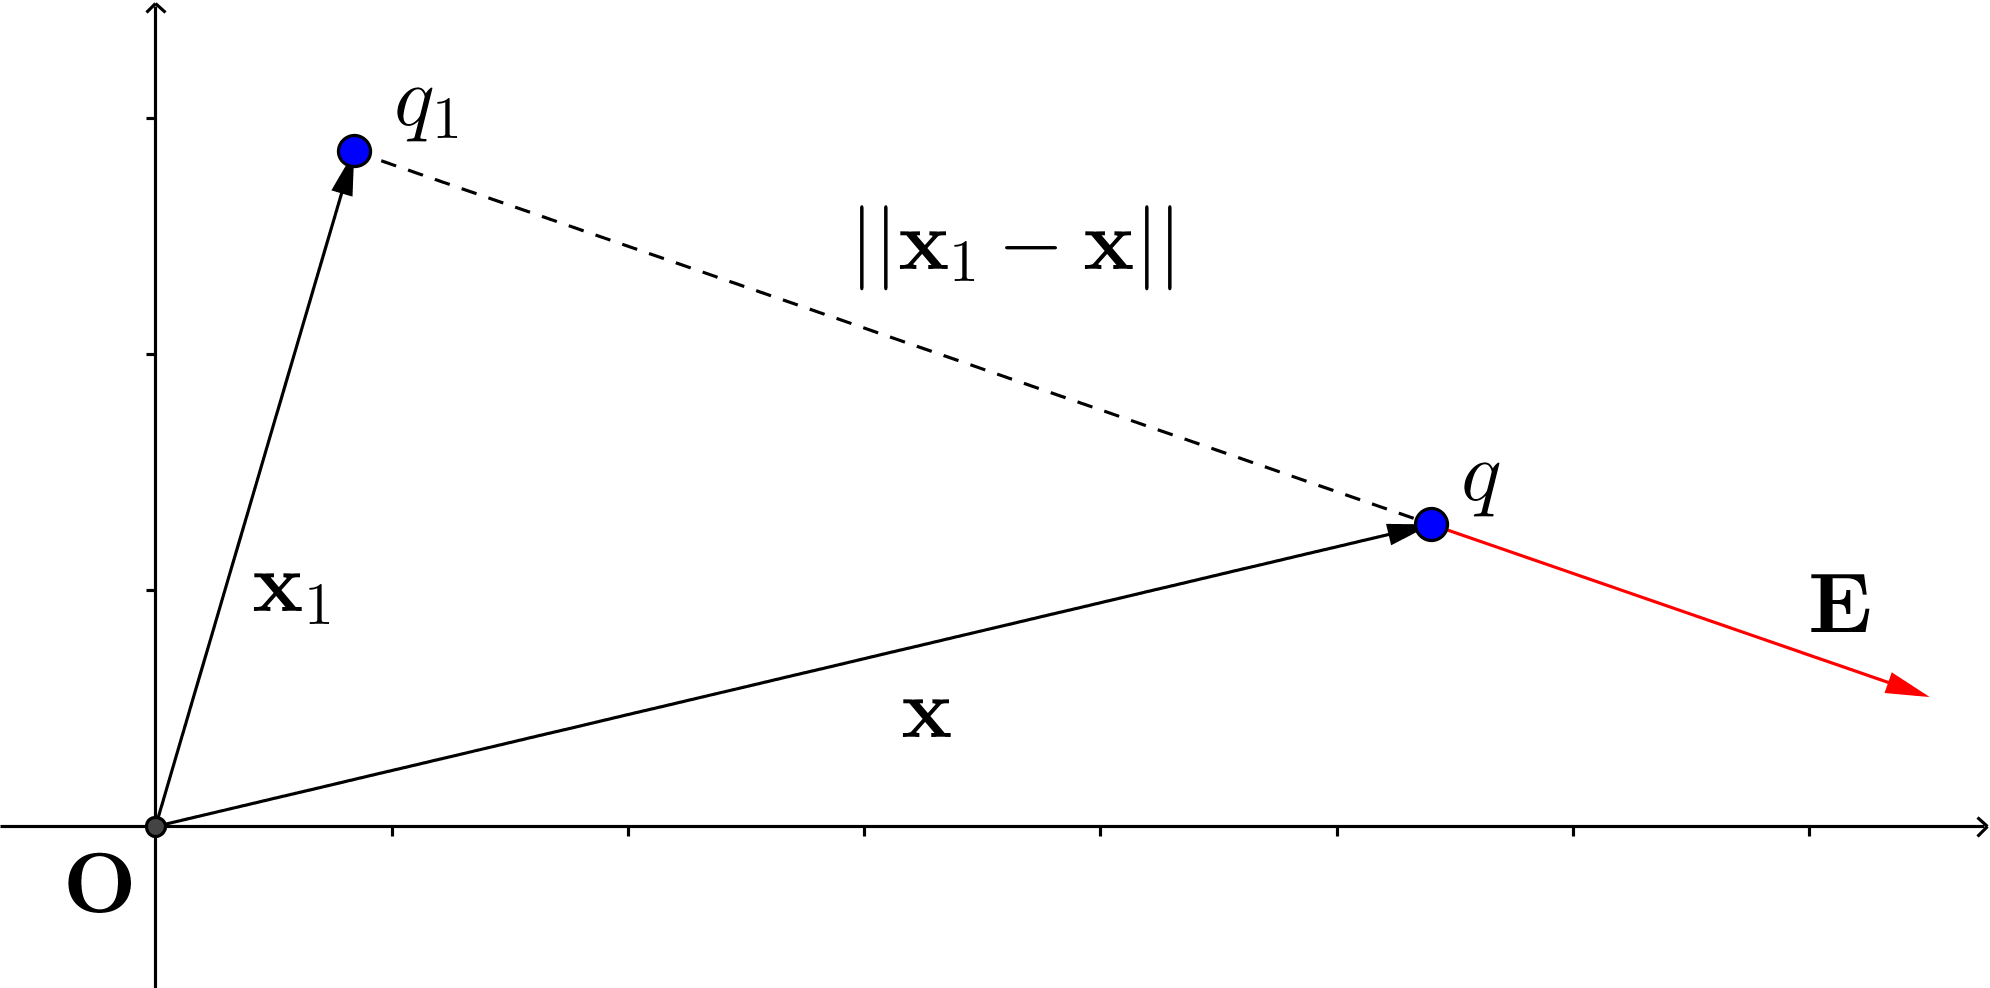
\includegraphics[scale=1.5]{camp_elet}
\caption{\textit{Exemplificação da interação entre cargas elétricas devido à geração, em função de $q_1$ (positiva), de um campo elétrico. A força elétrica $\textbf{F}$ atuando numa carga qualquer $q$ tem mesma direção do campo elétrico $\textbf{E}$, com mesmo sentido ou sentido oposto conforme a carga $q$ é positiva ou negativa, respectivamente.}}
\label{fig.camp_eletr}
\end{figure}

%\begin{figure}[!htb]
%\centering
%\subfloat{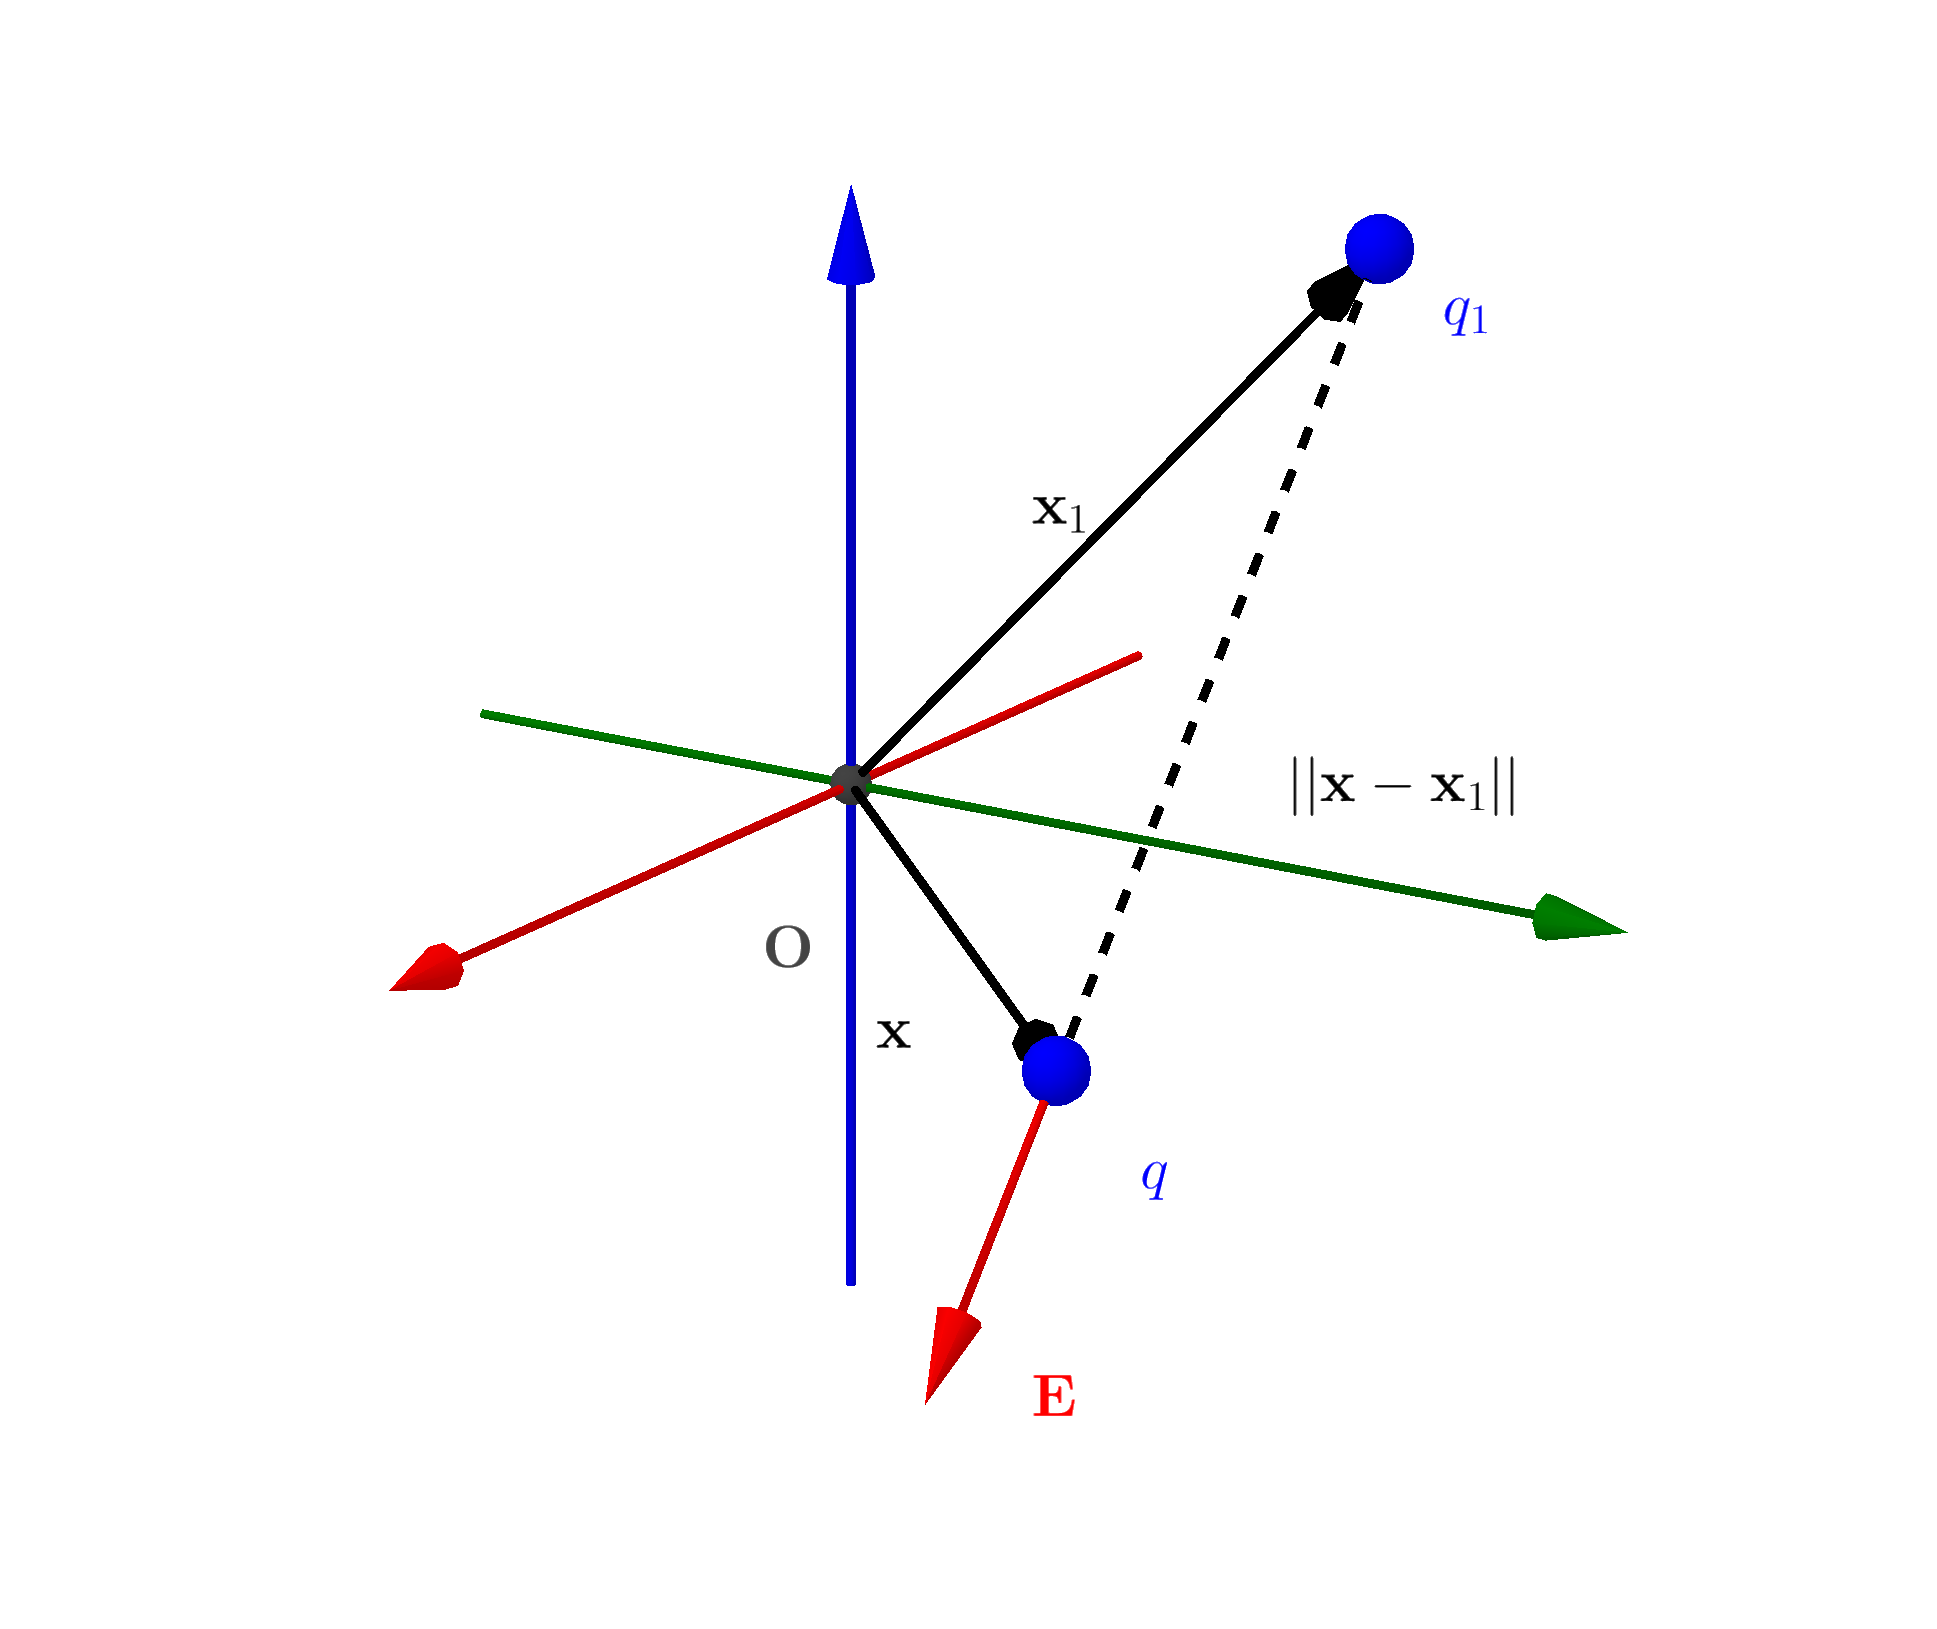
\includegraphics[scale=1]{camp_elet_3D}}
%\subfloat{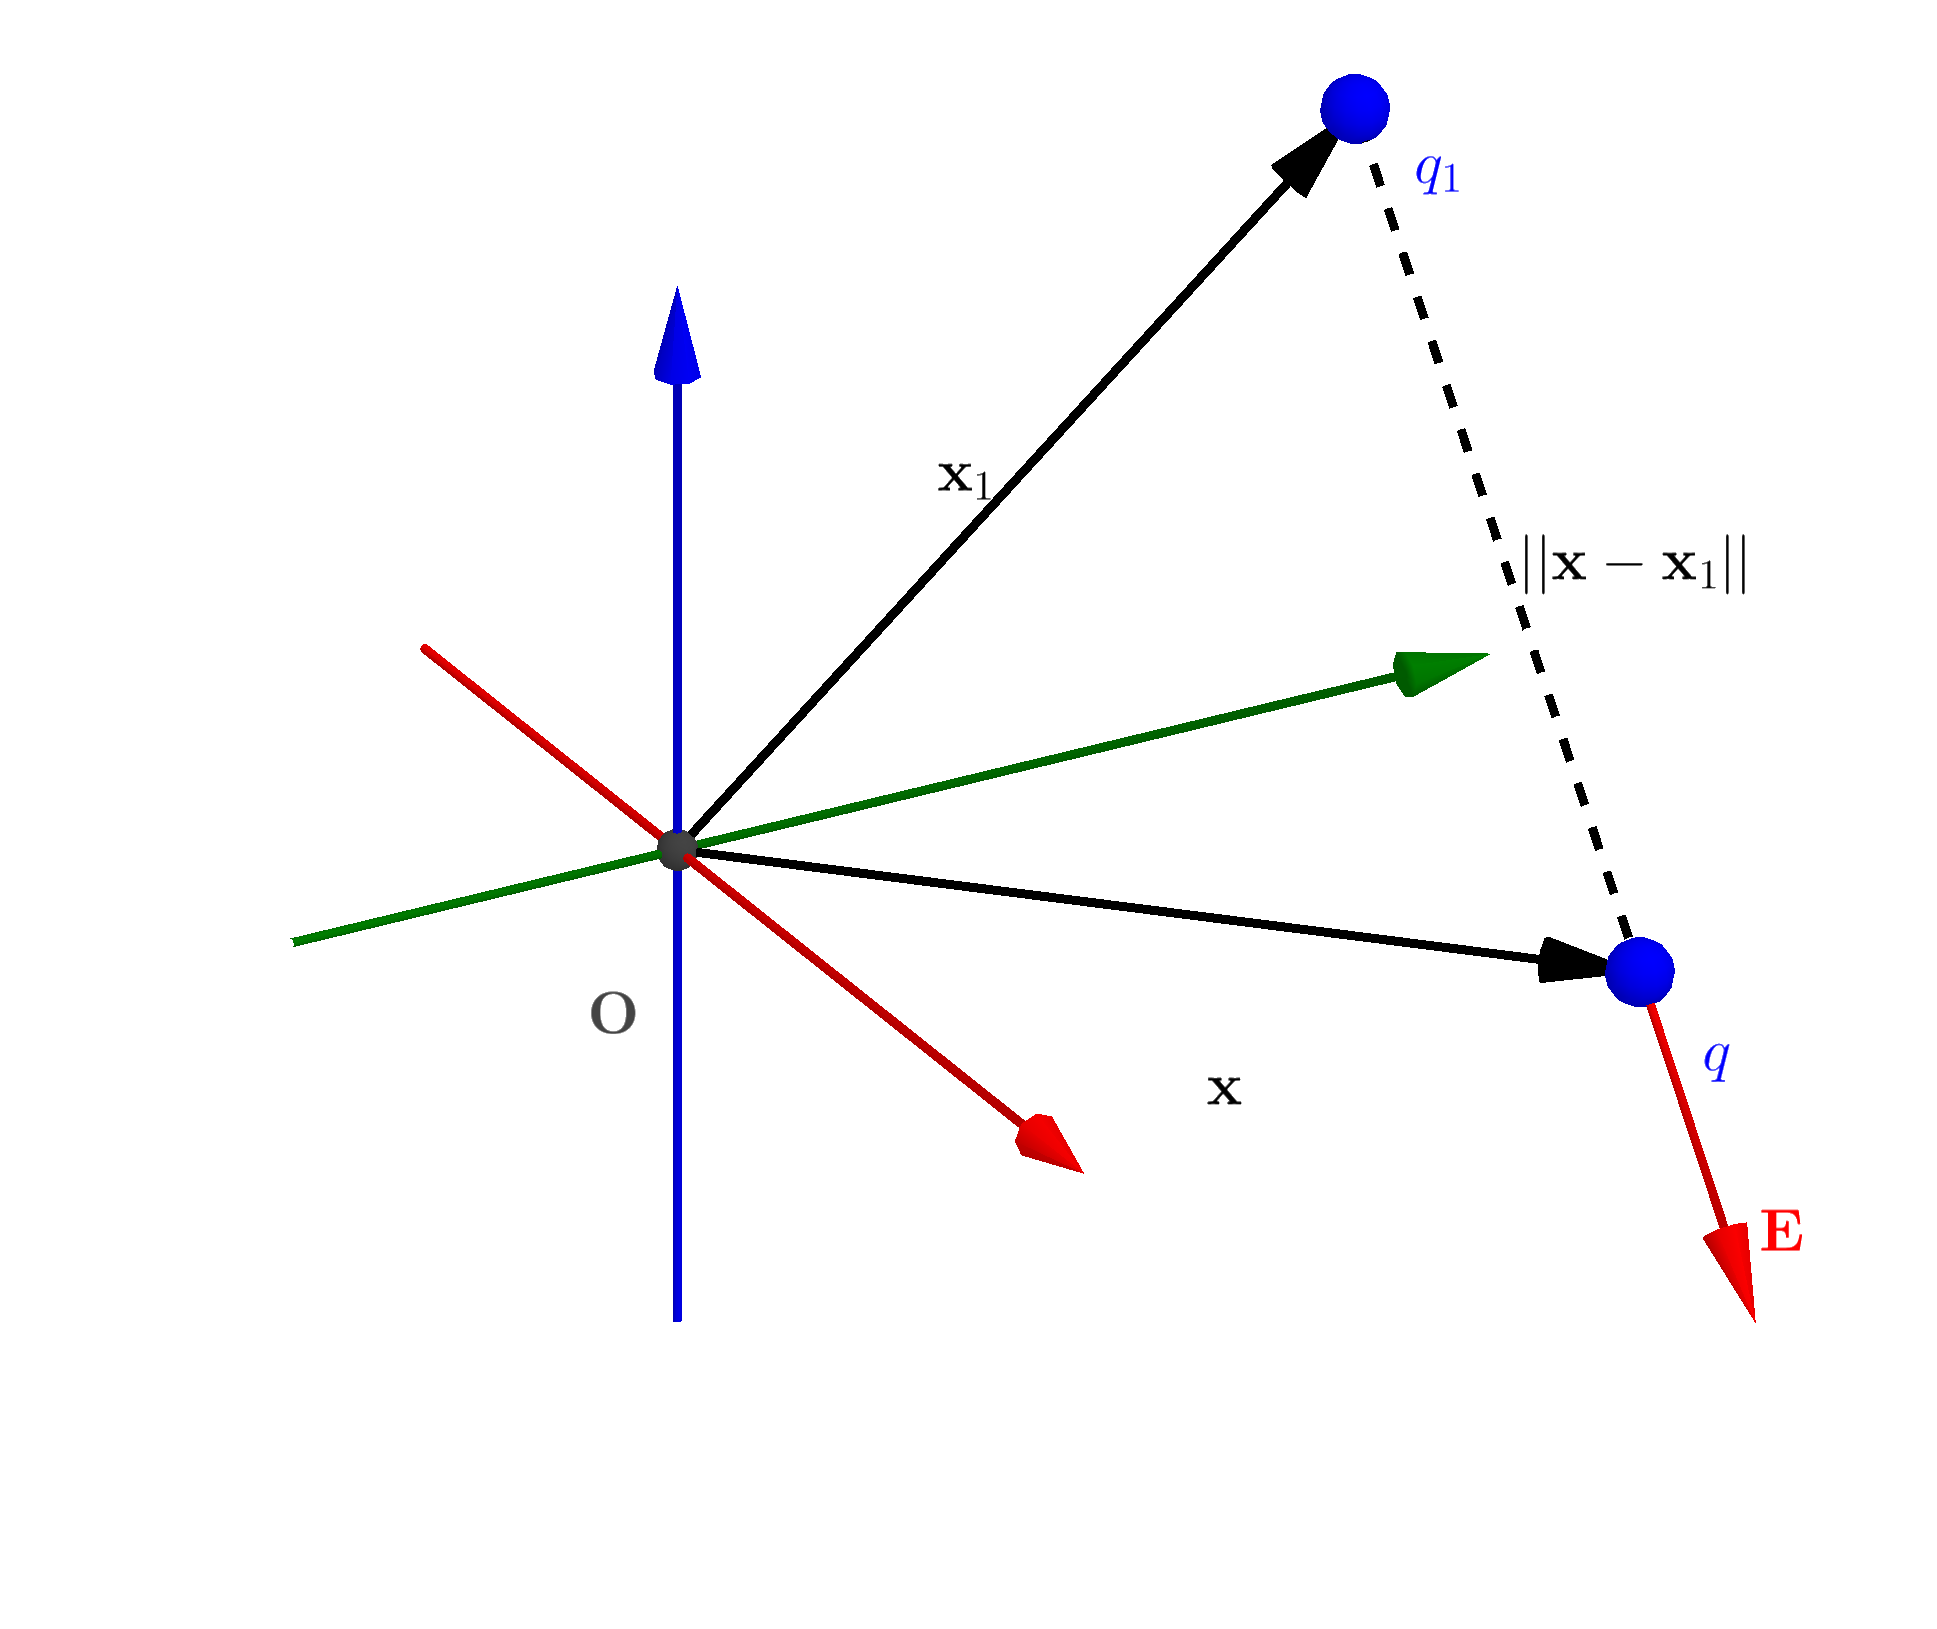
\includegraphics[scale=1]{camp_elet_3D2}}
%\caption{}
%\label{fig.mossul}
%\end{figure}

Num sistema com mais de uma carga fonte produzindo campos elétricos, foi observado experimentalmente que o campo elétrico total atuando num ponto $\textbf{x}$ é simplesmente o somatório dos campos produzidos por cada carga, o que ficou conhecido como a \textit{Superposição Linear} e pode ser expressada na forma
\begin{equation*}
\textbf{E}=k\,\sum_{i=1}^{n}q_i\,\frac{\textbf{x}_i-\textbf{x}}{||\textbf{x}_i-\textbf{x}||^3}.
\end{equation*} 
O campo elétrico devido a um pequeno número de cargas pode ser calculado a partir do princípio da superposição linear. Mas se temos uma quantidade muito grande de cargas num determinado volume $V$, devemos calcular a \textit{densidade volumétrica de carga elétrica} $\rho$ num volume infinitesimal situado em $\textbf{x}_0$ e em seguida integrar sobre o volume $V$ para obter a quantidade total de carga $Q$. A densidade de carga é definida por
\begin{equation*}
\rho(\textbf{x}_0)=\lim_{\Delta V_i \to 0}\frac{\Delta q_i}{\Delta V_i}=\frac{d\,q}{d\,V},
\end{equation*}
medida, no SI, em $C/m^3$. A quantidade total de carga $Q=\sum_i \Delta\,q_i$ no volume $V$ é
\begin{equation}\label{eq.densidade_carga}
Q=\iiint_{V}\rho(\textbf{x}_0)\,dV.
\end{equation}

O \textit{fluxo elétrico} é definido como a quantidade linhas do campo elétrico que atravessam uma superfície qualquer, e é dado pela equação
\begin{equation*}
\Phi_\textbf{E}=\textbf{E}\cdot\textbf{A}. 
\end{equation*} 
O \textit{vetor área} é definido como a magnitude da área da superfície atravessada apontando na direção do vetor normal à superfície, $\textbf{A}=A\,\textbf{n}$, e estamos considerando um campo elétrico uniforme $\textbf{E}$ que se desloca na direção $\textbf{n}$, ou seja, é perpendicular à superfície $A$ como podemos observar na figura \ref{fig.flux_ele}.
\begin{figure}[!htb]
\centering
\subfloat{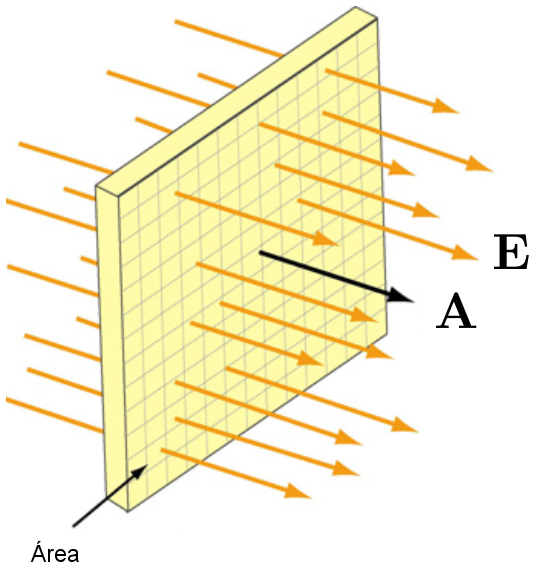
\includegraphics[scale=.4]{campo_area_2}}
\quad
\subfloat{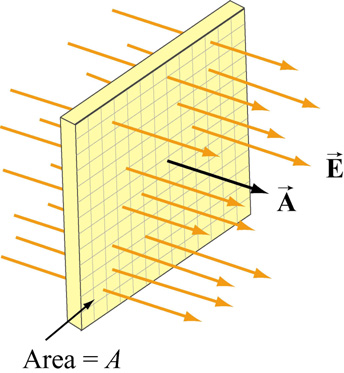
\includegraphics[scale=.4]{campo_area}}
\caption{\textit{Fluxo elétrico, linhas de campo elétrico passando através de uma superfície.}}
\label{fig.flux_ele}
\end{figure}
Mas se o campo elétrico se propaga formando um ângulo $\theta$ com o vetor normal da superfície, então o fluxo elétrico é dado por
\begin{equation*}
\Phi_\textbf{E}=\textbf{E}\cdot\textbf{A}=E\,A\,\cos\theta,
\end{equation*}
com $E=\textbf{E}\cdot\textbf{n}$ sendo a componente do campo elétrico na direção $\textbf{n}$. Em geral uma superfície $S$ pode ser curva e estamos interessados numa superfície \textit{fechada}, ou seja, aquela que engloba um determinado volume, o qual contém uma carga elétrica (exemplo na figura \ref{fig.esfe_gauss}). Tomando uma área bem pequena dessa superfície, $\Delta\textbf{A}_i$, o campo elétrico pode ser variável em cada parte da superfície e nessas condições temos que o fluxo nessa pequena região é dado por
\begin{equation*}
\Delta\,\Phi_\textbf{E}=\textbf{E}_i\cdot\Delta\,\textbf{A}_i.
\end{equation*}
O fluxo positivo atravessando toda a superfície de dentro para fora é calculado tomando o limite quando $\Delta\textbf{A}_i\to 0$ e aumentando infinitamente a quantidade dessas pequenas áreas até cobrir a superfície $S$
\begin{equation}\label{eq.fluxo_eletr}
\Phi_\textbf{E}=\lim_{i\to\infty}\sum_i\textbf{E}_i\cdot\textit{d}\textbf{A}_i=\oiint_S\textbf{E}\cdot\textit{d}\textbf{A}.
\end{equation}

Considere uma carga pontual positiva $q$ localizada no centro de uma esfera imaginária de raio $r$, onde essa carga produz um campo elétrico que aponta na direção radial conforme a figura \ref{fig.esfe_gauss}. Sabemos que a área da superfície dessa esfera é dada por $A=4\pi\,r^2$ e que, segundo a equação \ref{eq.campo_eletrico}, a magnitude do campo elétrico em qualquer ponto da superfície esférica é
\begin{equation*}
E=\frac{q}{4\pi\epsilon_0\,r^2},
\end{equation*}
assim o fluxo elétrico é calculado usando a equação \ref{eq.fluxo_eletr}.
\begin{align*}
\Phi_\textbf{E}&=\oiint_S\textbf{E}\cdot\textit{d}\textbf{A}\\
&=\oiint_S\textbf{E}\cdot\textbf{n}\,\textit{d}A\\
&=E\,\oiint_S\textit{d}A\\
&=E\,A\\
&=\frac{q}{4\pi\epsilon_0\,r^2}\,4\pi\,r^2\\
&=\frac{q}{\epsilon_0}.
\end{align*}
Na demonstração acima escolhemos uma esfera como \textit{superfície Gaussiana} mas, introduzindo o conceito de \textit{ângulo sólido}, vemos que a demonstração é válida para qualquer superfície fechada, utilizada em aplicações que apresentem mais ou menos alguma simetria (esférica, planar ou cilíndrica). Para mais detalhes consultar \cite{jackson_classical_1999}. Assim, concluímos que o fluxo elétrico através de uma superfície fechada que apresente mais ou menos alguma simetria é diretamente proporcional à quantidade de carga enclausurada pela superfície. Matematicamente, a \textit{lei de Gauss} para o fluxo elétrico é
\begin{equation}\label{eq.fluxo_eletrico}
\Phi_\textbf{E}=\oiint_S\textbf{E}\cdot\textit{d}\textbf{A}=\frac{q}{\epsilon_0}.
\end{equation}
\begin{figure}[!htb]
\centering
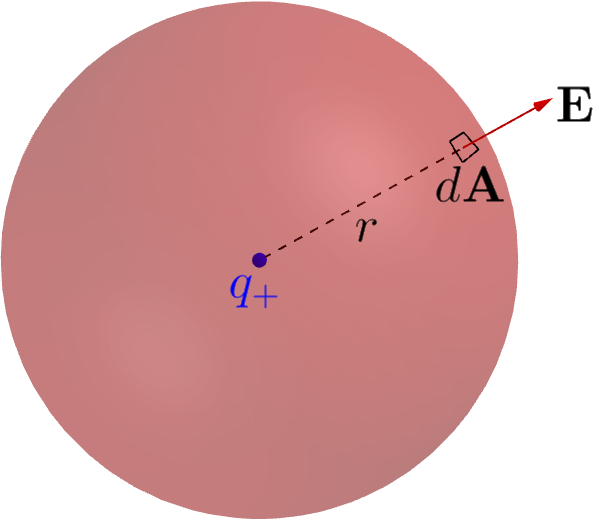
\includegraphics[scale=.3]{esfera_gaussiana}
\caption{\textit{Esfera Gaussiana enclausurando uma carga positiva $q$. Nessas condições, o ângulo entre o vetor campo elétrico e o vetor normal à superfície infinitesimal $d\textbf{A}$ é zero.}}
\label{fig.esfe_gauss}
\end{figure}

Uma carga elétrica produz um campo elétrico, e de maneira similar uma barra magnética, ou ímã, produz um \textit{campo magnético} $\textbf{B}$. Um ímã possui um polo norte de onde partem as linhas de campo magnético e um polo sul por onde as linhas de campo magnético retornam ao ímã (figura \ref{fig.barras_mag}). Diferentemente das cargas elétricas que são observadas isoldamente na natureza, os dois polos magnéticos sempre aparecem aos pares, ou seja, monopolos magnéticos não existem isoladamente apesar de a suposição de sua existência ser de interesse teórico. Assim, sempre que um ímã é fracionado, mesmo que em partes muito elementares, o resultado sempre será um novo ímã com dois polos magnéticos conforme a figura \ref{fig.barras_mag}.
\begin{figure}[!htb]
\centering
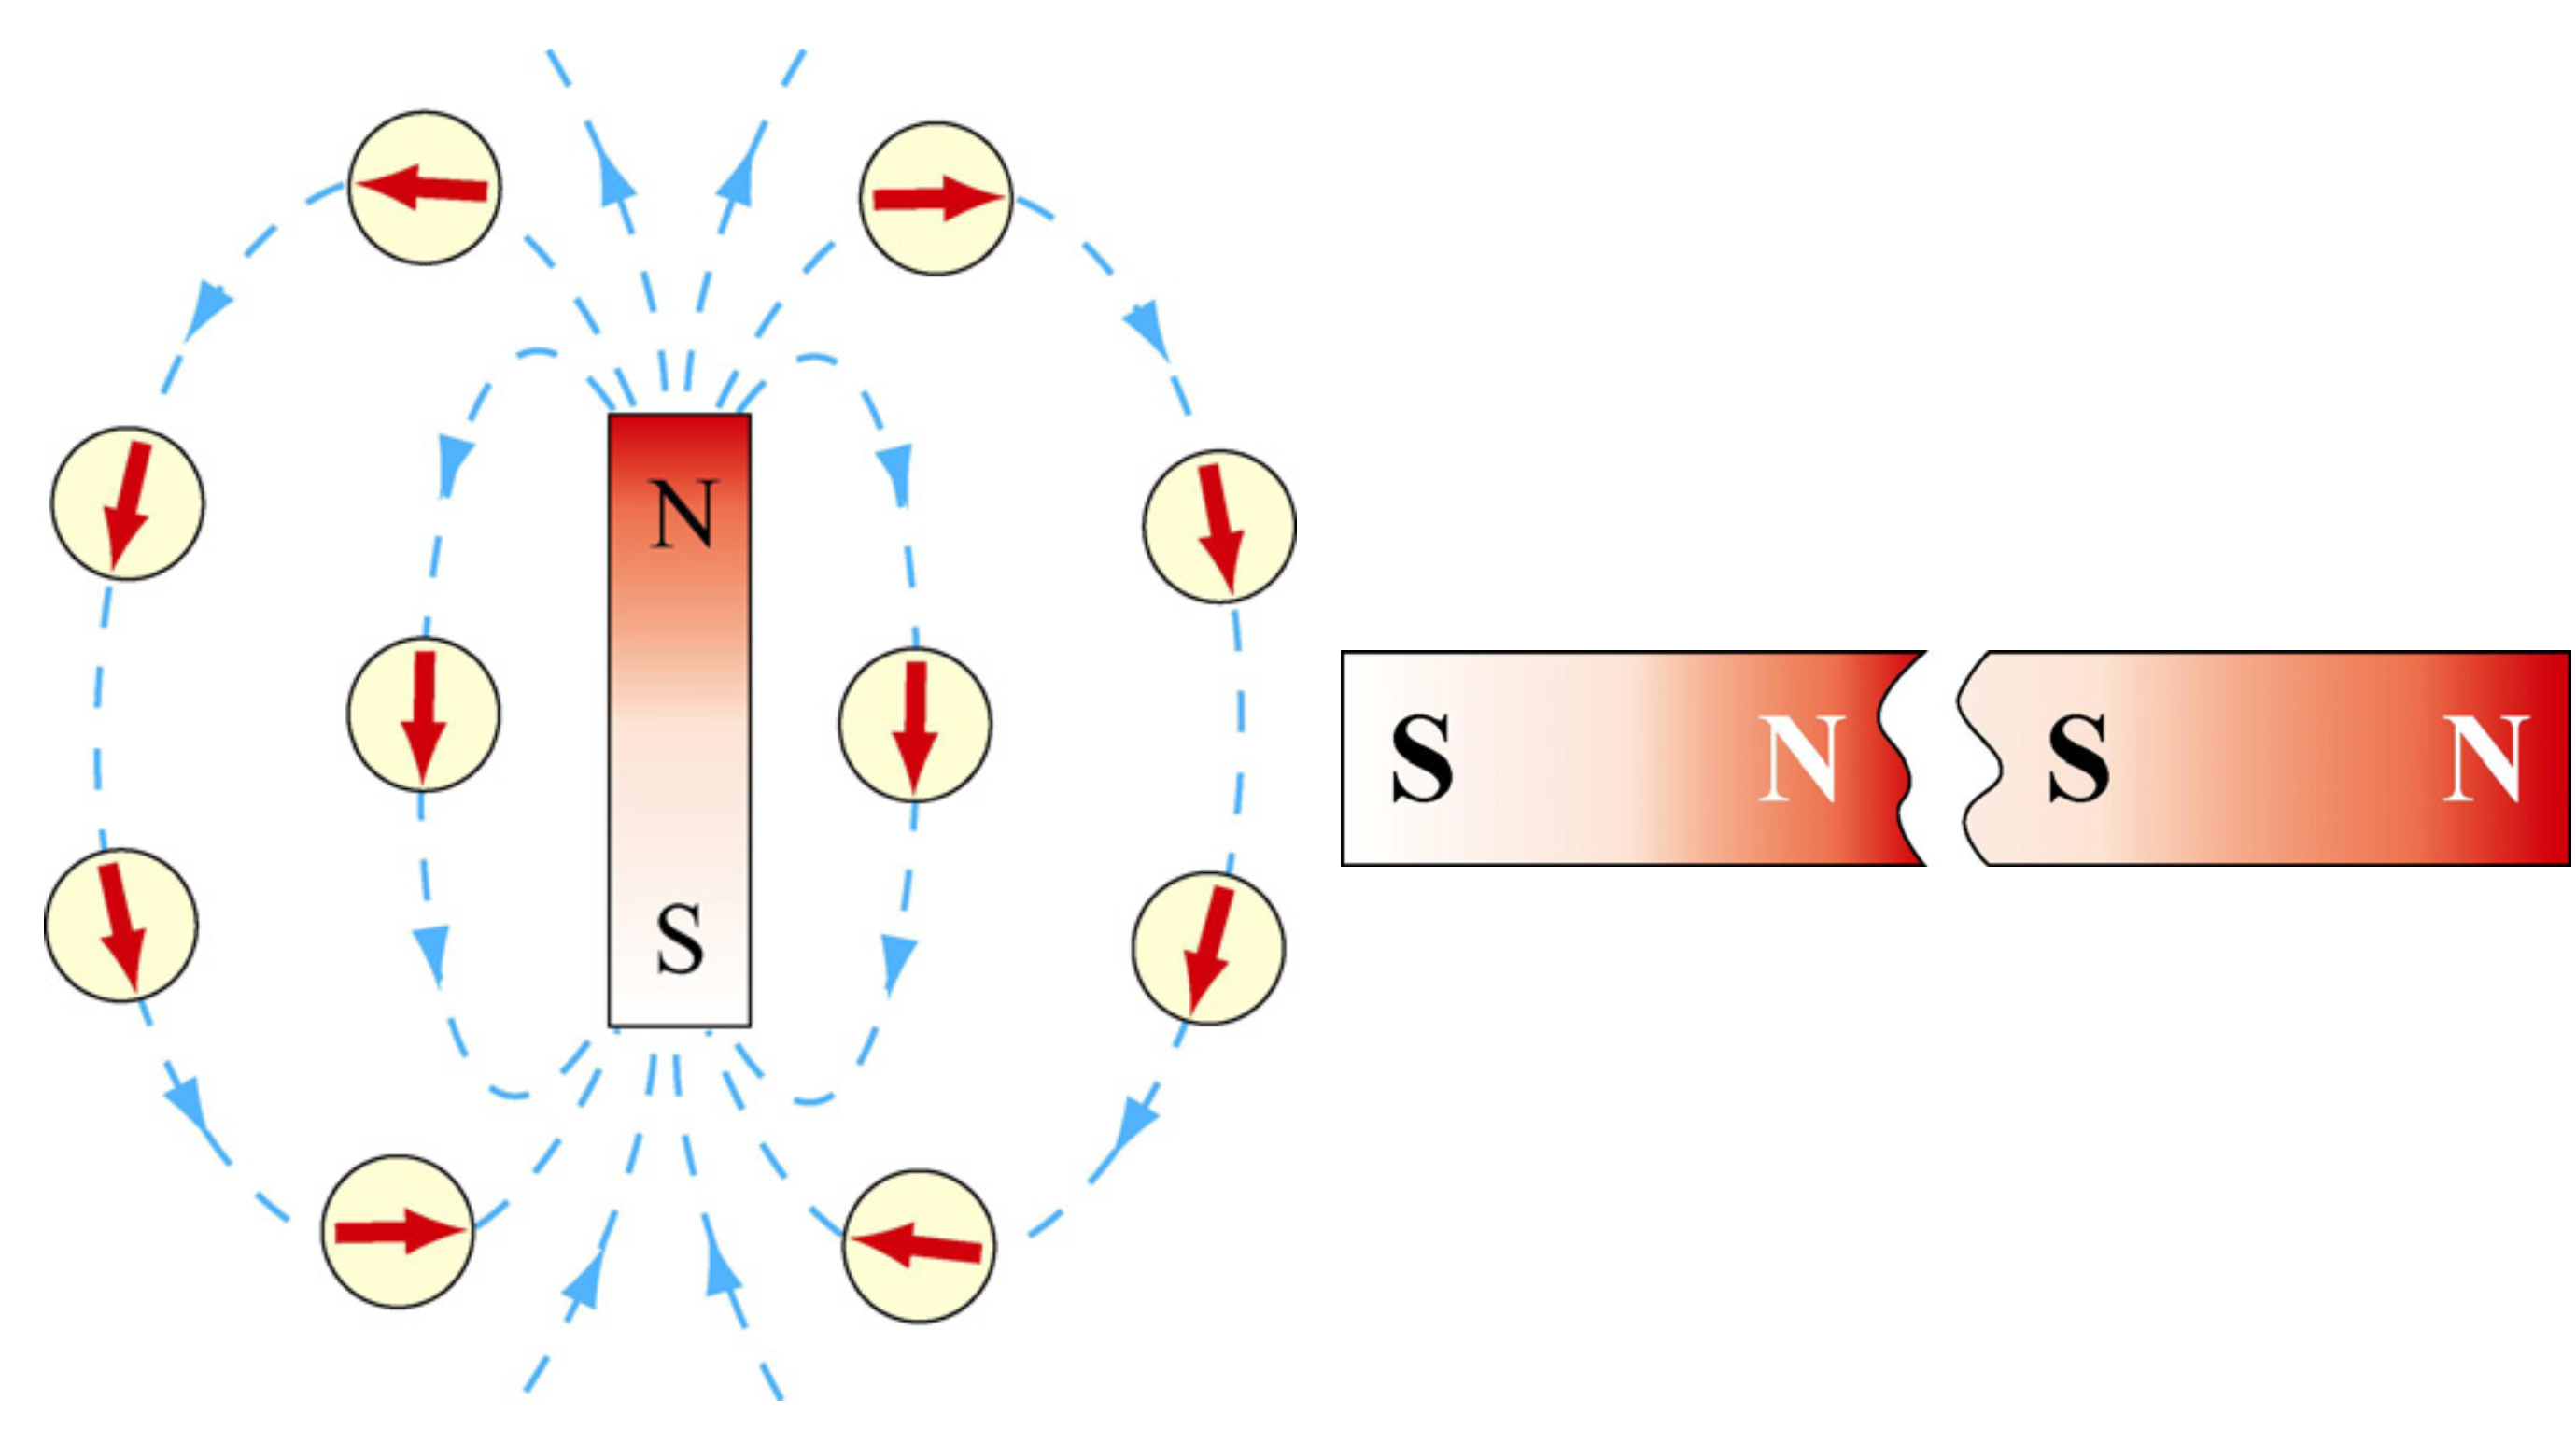
\includegraphics[scale=.7]{barras_magn}
\caption{\textit{Barras magnéticas onde polos de mesmo sinal se repelem e polos de sinais contrários se atraem.}}
\label{fig.barras_mag}
\end{figure}
Como não existem monopolos magnéticos, o campo magnético deve ser definido de forma diferente do campo elétrico, e experimentalmente foram observadas algumas características relacionadas ao movimento de uma carga elétrica $q$ com velocidade $\textbf{v}$ num campo magnético $\textbf{B}$:
\begin{itemize}
\item a magnitude da força magnética $\textbf{F}_B$ é proporcional à $v$, $B$ e $q$, onde $v$ e $B$ são as magnitudes da velocidade e do campo magnético respectivamente,
\item a direção de $\textbf{F}_B$ é perpendicular ao plano formado por $\textbf{v}$ e $\textbf{B}$,
\item $\textbf{F}_B$ é proporcional ao $\sin\theta$, o ângulo formado por $\textbf{v}$ e $\textbf{B}$. Se $\textbf{v}$ e $\textbf{B}$ são paralelos então $\textbf{F}_B=0$, e
\item o sentido de $\textbf{F}_B$ depende do sinal da carga $q$.
\end{itemize}
Essas observações são ilustradas na figura \ref{fig.froca_mag_veloc} e a força magnética é definida como
\begin{equation*}
\textbf{F}_B=q\,\textbf{v}\times\textbf{B}.
\end{equation*}
\begin{figure}[!htb]
\centering
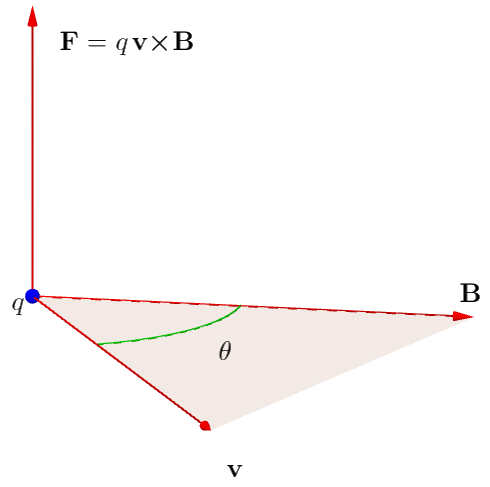
\includegraphics[scale=.4]{forca_camp_mag_veloc}
\caption{\textit{Força magnética agindo numa carga elétrica que se desloca num campo magnético.}}
\label{fig.froca_mag_veloc}
\end{figure}
Teoricamente, poderíamos tentar determinar a lei de Gauss para o fluxo magnético com o mesmo procedimento aplicado ao fluxo elétrico e obter
\begin{equation*}
\Phi_\textbf{B}=\oiint_S\textbf{B}\cdot\textit{d}\textbf{A}=\frac{q_m}{\mu_0},
\end{equation*} 
onde $q_m$ é a carga magnética (suposto monopolo magnético) enclausurado pela superfície Gaussiana, $\mathbf{B}$ é o campo magnético e $\mu_0$ é a \textit{permeabilidade magnética no vácuo} com valor $\mu_0=4\,\pi\times 10^{-7}\, T\,m/A$. No entanto, não foi constatada a existência de qualquer carga magnética isolada mesmo após muitos esforços. Como $q_m=0$, temos que a lei de Gauss para o magnetismo é
\begin{equation}\label{eq.gauss_flux_mag}
\Phi_\textbf{B}=\oiint_S\textbf{B}\cdot\textit{d}\textbf{A}=0.
\end{equation}
Conforme podemos ver na figura \ref{fig.flux_elet_magn}, a equação \ref{eq.gauss_flux_mag} implica que a quantidade de linhas do campo magnético saindo da superfície é igual à quantidade que está entrando, ou seja, não há uma origem isolada e um término isolado para o fluxo magnético como há para o fluxo elétrico. Outro problema é que a barra imantada atravessa a superfície que, de acordo com a hipóteses da lei de Gauss, deveria ser fechada.
\begin{figure}[!htb]
\centering
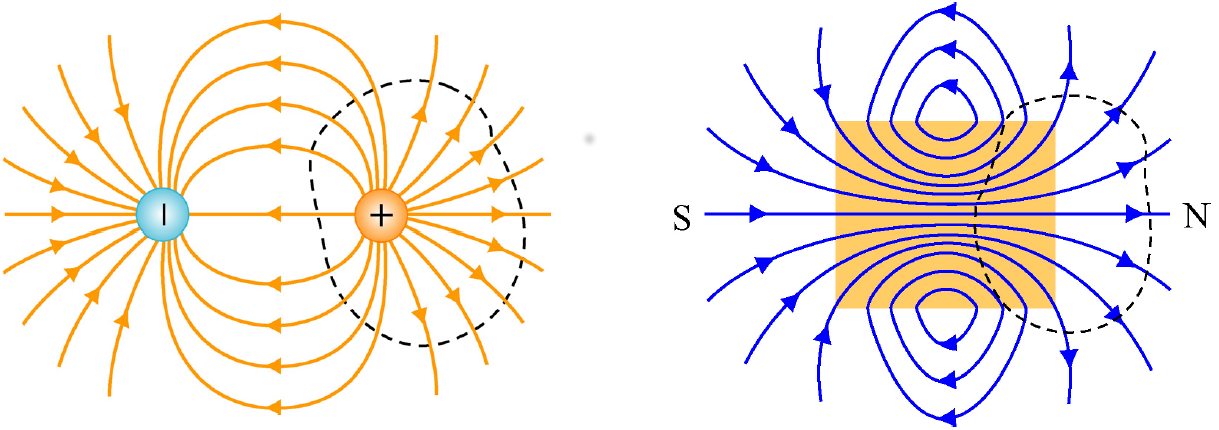
\includegraphics[scale=.3]{flux_ele_mag}
\caption{\textit{As linhas do campo magnético que emanam do polo norte do ímã em direção ao polo sul retornam para dentro da superfície Gaussiana descrevendo um laço fechado.}}
\label{fig.flux_elet_magn}
\end{figure}

\subsection{A Lei de Ampère}\label{sec.lei_ampere}
Correntes elétricas podem ser produzidas por cargas elétricas que se movem num fio condutor. Essas correntes elétricas são fontes de campos magnéticos $d\,\textbf{B}$, num determinado ponto $\mathbf{x}$, e que podem ser calculados em função da corrente $I$ num intervalo infinitesimal $d\,\textbf{l}$ do fio. Visualização na figura \ref{fig.corrente_fio}. A fonte de corrente infinitesimal é dada por $I\,d\,\textbf{l}$ e $r$ é a distância entre o ponto de aplicação do campo magnético e a fonte de corrente infinitesimal. O vetor $\textbf{n}$ é o vetor normal que aponta na direção de $\mathbf{x}$ e o vetor $d\,\textbf{l}$ aponta na direção e sentido da corrente $I$. Repare ainda que o campo magnético depende do ângulo $\theta$ entre $\mathbf{n}$ e $d\mathbf{l}$.
\begin{figure}
\centering
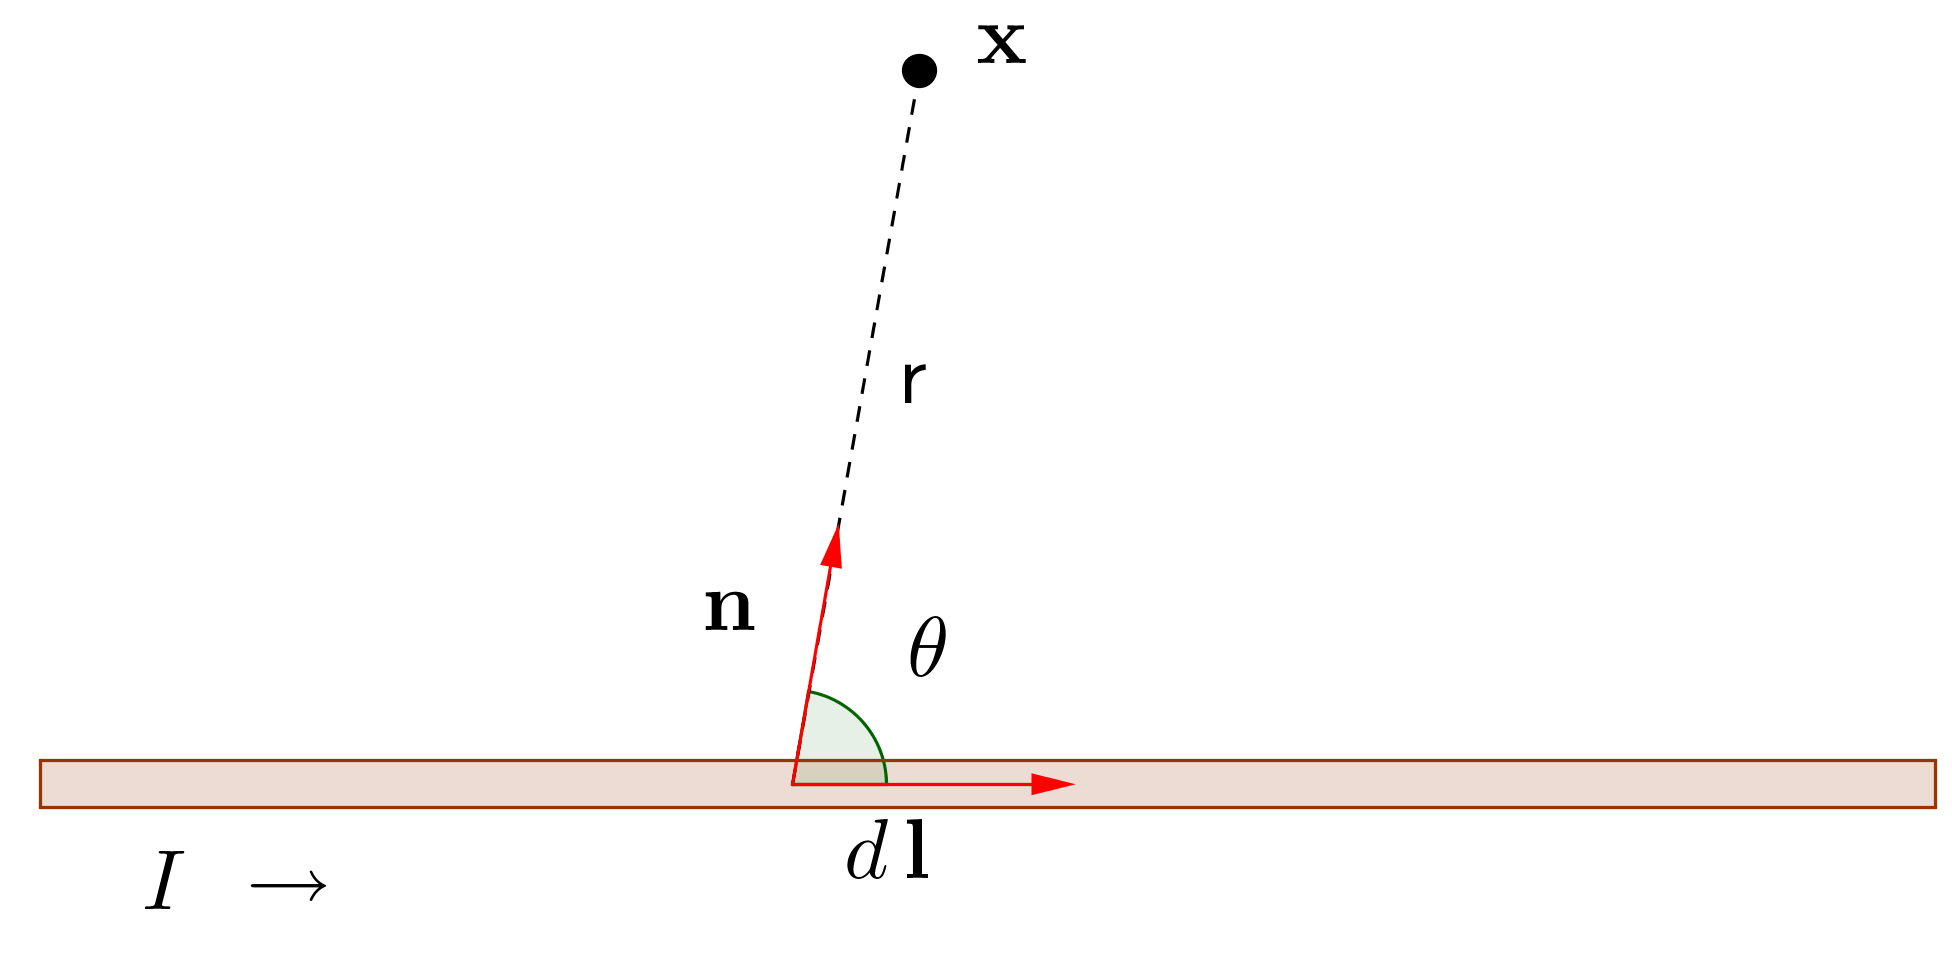
\includegraphics[scale=1.1]{corrente_fio}
\caption{\textit{Campo magnético no ponto $\mathbf{x}$ devido a passagem de uma corrente elétrica $I$ pelo fio. Observe que a magnitude do campo depende também do ângulo $\theta$ entre $\textbf{l}$ e $\textbf{n}$}.}
\label{fig.corrente_fio}
\end{figure}
Assim sendo, a \textit{Lei de Biot-Savart} tem definição análoga à do campo elétrico (derivada da lei de Coulomb) e pode ser expressa como
\begin{equation}\label{eq.lei_biot_savart}
d\,\textbf{B}=\frac{\mu_0}{4\,\pi}\frac{I}{r^2}\,d(\textbf{l}\times\textbf{n}),
\end{equation}
e o campo magnético no volume ao redor do fio pode ser obtido integrando sobre a direção perpendicular ao plano formado por $\textbf{l}$ e $\textbf{n}$ ao longo do comprimento do fio.
\begin{equation}
\textbf{B}=\frac{\mu_0I}{4\,\pi}\int_{\textbf{l}}\frac{d(\textbf{l}\times\textbf{n})}{r^2}.
\end{equation}

Considere agora um laço circular (linha de campo magnético) de raio $r$ contido num plano perpendicular ao fio condutor, onde esse laço está dividido em pequenos comprimentos $\Delta\textbf{s}=\Delta s\,\pmb{\phi}$, cujos vetores correspondentes a cada ponto do laço apontam na direção do vetor tangencial à circunferência naquele ponto, conforme  a figura \ref{fig.laco_amperiano}. Esse laço fechado contido num plano é denominado \textit{laço Amperiano} e é usado para calcular o campo magnético referente àquela linha de campo tomando o limite quando $\Delta\textbf{s}\to 0$ e integrando no intervalo dado pelo comprimento da circunferência. Nesse caso, $\theta=\pi$ e $\pmb{\phi}$ é perpendicular ao plano formado por $\textbf{l}$ e $\textbf{n}$, portanto a magnitute do vetor  $\textbf{B}$ na direção $\pmb{\phi}$ é dada pela lei de Biot-Savart na equação \ref{eq.lei_biot_savart}.
\begin{equation*}
\oint_{s}\textbf{B}\cdot d\textbf{s}=B\oint_{s}ds=\frac{\mu_0I}{2\pi\,r}2\pi\,r=\mu_0I.
\end{equation*} 
\begin{figure}[h]
\centering
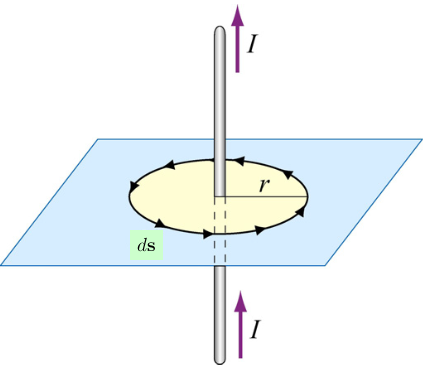
\includegraphics[scale=.4]{laco_amperiano}
\caption{\textit{Laço amperiano seguindo a regra da mão direita: posicionando o polegar no sentido da corrente, o campo magnético tem o mesmo sentido dos demais dedos curvando em torno do fio.}}
\label{fig.laco_amperiano}
\end{figure}

Vamos considerar um outro exemplo de laço amperiano cujo contorno denotado por $abcda$ se sobrepõe a duas linhas de campo magnético coplanares, observado na figura \ref{fig.laco_amper_2}. No desenvolvimento abaixo, a primeira e terceira integrais zeram pois o campo magnético é perpendicular ao caminho de integração nesses intervalos, e $B_2(r_2\theta)$ e $B_1[r_1(2\pi-\theta)]$ são os comprimentos dos arcos $bc$ e $da$, respectivamente. A integral de linha do campo magnético no contorno $abcda$ é
\begin{align*}
\oint_{abcda}\textbf{B}\cdot d\textbf{s}&=\oint_{ab}\textbf{B}\cdot d\textbf{s}+\oint_{bc}\textbf{B}\cdot d\textbf{s}+\oint_{cd}\textbf{B}\cdot d\textbf{s}+\oint_{da}\textbf{B}\cdot d\textbf{s}\\
&=0+B_2(r_2\theta)+0+B_1[r_1(2\pi-\theta)]\\
&=\frac{\mu_0I}{2\pi\,r_2}(r_2\theta)+\frac{\mu_0I}{2\pi\,r_1}[r_1(2\pi-\theta)]\\
&=\frac{\mu_0I}{2\pi}\theta+\frac{\mu_0I}{2\pi}(2\pi-\theta)\\
&=\mu_0I.
\end{align*}
\begin{figure}
\centering
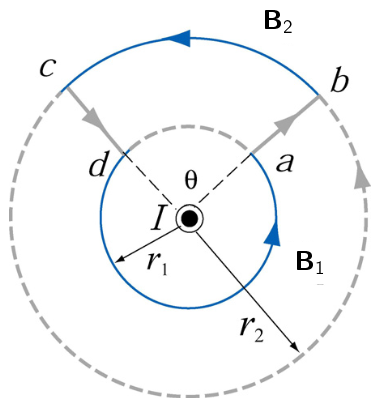
\includegraphics[scale=.5]{laco_amperiano_2}
\caption{\textit{Laço amperiano passando por duas linhas de campo magnético. O ponto no centro significa que o sentido da corrente elétrica está ``saindo do plano do papel".}}
\label{fig.laco_amper_2}
\end{figure}
Vemos o mesmo resultado se o laço amperiano envolve uma ou duas linhas de campo magnético e, usando coordenadas cilíndricas, podemos demonstrar que o mesmo resultado é válido para uma quantidade arbitrária de linhas de campo magnético, ou seja, a integral de linha do campo magnético através de qualquer laço amperiano fechado é proporcional à corrente elétrica inscrita no laço. A \textit{Lei de Ampère} é dada por
\begin{equation*}
\oint_{s}\textbf{B}\cdot d\textbf{s}=\mu_0I.
\end{equation*}
Analogamente à lei de Gauss para campos elétricos, para ser aplicada a lei de Ampère é necessário que o laço possua alguma simetria em relação ao fio. No caso de um fio condutor suficientemente comprido para que suas extremidades não interfiram na aplicação, temos uma simetria cilíndrica e a lei de Ampère pode ser aplicada normalmente. Caso o fio não seja suficientemente comprido, devemos utilizar a lei de Biot-Savart. 

Agora considere a seguinte situação, descrita por Maxwell, onde o circuito elétrico está interrompido por um capacitor. 
\begin{figure}
\centering
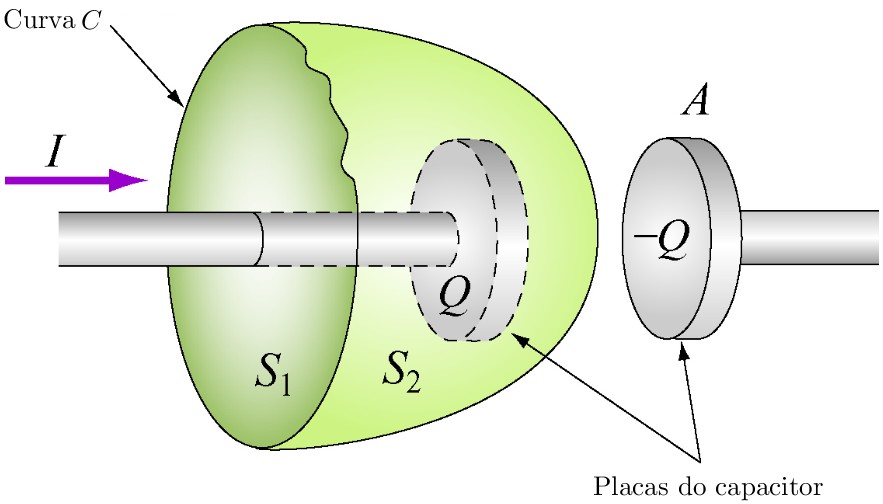
\includegraphics[scale=.3]{capacitor}
\caption{\textit{Quando há corrente no circuito, cargas positivas se acumulam numa placa do capacitor assim como cargas negativas se acumulam na outra placa. Tal acúmulo gera um fluxo elétrico variável entre as placas.}}
\label{fig.capacitor}
\end{figure}
Como vimos pela lei de Ampère, o campo magnético depende somente da corrente no circuito e do comprimento da circunferência que limita a superfície atravessada pelo fio condutor, e não depende dessa superfície em si. Portanto, o campo magnético referente à curva $C$ da figura \ref{fig.capacitor} pode ser calculado considerando a superfície $S_1$ ou a superfície $S_2$. A superfície $S_1$ é atravessada pela corrente $I$ a qual produz o campo magnético $\mathbf{B}$, mas superfície $S_2$ não é atravessada por $I$ e, no entanto, é produzido o mesmo campo magnético $\mathbf{B}$. Assim podemos sugerir que exista um outro fenômeno físico entre as placas do capacitor que seja responsável pela geração de $\mathbf{B}$. À medida que o capacitor vai sendo carregado, cargas elétricas opostas vão se acumulando em suas placas gerando um campo elétrico variável entre as placas, o qual produz um fluxo elétrico variável através da área da placa do capacitor. Maxwell mostrou que o produto da variação desse fluxo elétrico pela permissividade elétrica no vácuo era numericamente igual à corrente $I$, e por isso produzia o mesmo campo $\mathbf{B}$ quando integrado longo da curva $C$,
\begin{equation*}
I_d=\epsilon_0\frac{d\phi_E}{dt}.
\end{equation*}
Tal produto foi denominado \textit{corrente deslocada} e foi adicionado à lei de Ampère, a qual se tornou a \textit{lei de Ampére generalizada} ou \textit{lei de Ampère-Maxwell},
\begin{equation}\label{eq.ampere_generalizada}
\oint_s\mathbf{B}\cdot d\mathbf{s}=\mu_0I+\mu_0\epsilon_0\frac{d\phi_E}{dt}.
\end{equation}
Note que quando consideramos a superfície $S_1$, $I_d=0$ já que o fluxo elétrico é constante e assim $\mathbf{B}$ é dado somente por $I$. Quando consideramos a superfície $S_2$, $I=0$ e $\mathbf{B}$ é dado somente por $I_d$. 




\subsection{A Lei de Faraday}
Analogamente ao caso da força gravitacional, o \textit{trabalho} $W$ realizado por uma força elétrica $\textbf{F}_e$ para levar uma carga elétrica $q$ de um ponto $A$ até um ponto $B$ é definido como
\begin{equation}\label{eq.trabalho}
W=\int_{A}^{B}\textbf{F}_e\cdot d\textbf{s}.
\end{equation}
A diferença entre a \textit{energia potencial} $U$ em cada um dos pontos $A$ e $B$ é o que ocasiona o deslocamento da carga, assim a variação da energia potencial tem definição
\begin{equation}\label{eq.energia_potencial}
\Delta U=U_b-U_a=-\int_{A}^{B}\textbf{F}_e\cdot d\textbf{s}=-W.
\end{equation}
A \textit{diferença de potencial elétrico}, $\Delta V$, também chamada \textit{ddp}, é a variação da energia potencial por unidade de carga elétrica $q$. Utilizando a equação \ref{eq.camp_elet}, que relaciona força elétrica e campo elétrico, podemos definir a ddp como
\begin{equation}\label{eq.ddp}
\Delta V=-\int_{A}^{B}\frac{\textbf{F}_e}{q}\cdot d\textbf{s}=-\int_{A}^{B}\textbf{E}\cdot d\textbf{s}
\end{equation}
A ddp representa a quantidade de trabalho por unidade de carga para mover a carga do ponto $A$ ao ponto $B$ e sua unidade de medida no SI é o volt ($V=\frac{J}{C}$). Observe nas definições acima que só importa os valores no pontos $A$ e $B$, e não importa necessariamente o caminho que a carga vai percorrer de um ponto até o outro. 

Agora, num circuito elétrico fechado, as cargas percorrem um determinado caminho a partir de uma fonte de energia elétrica. Essa fonte é chamada de \textit{força eletromotriz}, representada por $\varepsilon$, e que pode ser pensada como uma ``bomba" de cargas que as impulsiona de um potencial menor para um potencial maior. A força eletromotriz é definida como o trabalho realizado para mover uma carga unitária na direção de maior potencial, matematicamente,
\begin{equation*}
\varepsilon=\frac{dW}{dq}, 
\end{equation*}
também medida em volt. Como o campo magnético não produz trabalho, o trabalho realizado sobre o movimento das cargas deve ser devido a um campo elétrico e para escrever a força eletromotriz em termos do campo elétrico de forma análoga ao que foi feito nas equações \ref{eq.trabalho}, \ref{eq.energia_potencial} e \ref{eq.ddp}, devemos utilizar uma integral de linha, pois nesse caso a corrente percorre um determinado caminho. Como o campo elétrico é não-conservativo (senão não haveria corrente) o valor da integral na equação \ref{eq.ddp} é diferente de zero. Assim,
\begin{equation}\label{eq.emf_E_nc}
\varepsilon=\oint_s\pmb{E}\cdot d\pmb{s}.
\end{equation}
 
O \textit{fluxo magnético} é definido de maneira similar ao fluxo elétrico e seu entendimento também pode ser acompanhado pela figura \ref{fig.flux_ele}. O fluxo magnético através de uma superfície é definido como
\begin{equation*}
\phi_\mathbf{B}=\textbf{B}\cdot\textbf{A}=B\,A\,\cos\theta,
\end{equation*}
onde o vetor área é $\textbf{A}=A\textbf{n}$, $\textbf{n}$ é o vetor normal à superfície atravessada, $A$ é a magnitude da área, $B=\textbf{B}\cdot\textbf{n}$ é a componente do campo magnético na direção do vetor normal e $\theta$ é o ângulo entre $\textbf{B}$ e $\pmb{A}$. Tomando um elemento infinitesimal da área e integrando sobre a superfície o fluxo magnético é
\begin{equation}\label{eq.fluxo_mag}
\phi_{\mathbf{B}}=\iint_S\mathbf{B}\cdot d\mathbf{A},
\end{equation}
medido em \textit{Weber}, $T/m^2$. 

Em 1831, Faraday descobriu que se pode criar um campo elétrico variando um campo magnético em função do tempo num fenômeno que foi batizado de \textit{indução eletromagnética}. Um dos experimentos de Faraday (figura \ref{fig.exper_faraday}) consiste em movimentar um ímã dentro de uma bobina feita de fio condutor onde se pode observar a geração de uma corrente elétrica, como se a bobina estivesse conectada a fonte de força eletromotriz. O experimento mostra que a força eletromotriz induzida é proporcional à taxa (negativa) de variação do fluxo magnético através da bobina, a \textit{lei de Faraday} é
\begin{equation*}
\varepsilon=-\frac{d\phi_\mathbf{B}}{dt}.
\end{equation*}
Podemos reescrever a lei de Faraday usando a equação \ref{eq.emf_E_nc},
\begin{equation}\label{eq.lei_faraday}
\varepsilon=\oint_s\pmb{E}\cdot d\pmb{s}=-\frac{d\phi_\mathbf{B}}{dt},
\end{equation}
o que implica que a variação do fluxo magnético induz um campo elétrico não-conservativo que varia com o tempo, diferente do campo elétrico conservativo gerado por cargas elétricas estacionárias.

\begin{figure}[!htb]
\centering
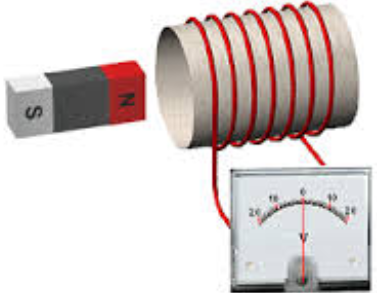
\includegraphics[scale=.5]{experi_faraday}
\caption{\textit{Experimento de indução eletromagnética promovido por Michael Faraday.}}
\label{fig.exper_faraday}
\end{figure}


\section{Equações de Maxwell}
Vimos pela equação \ref{eq.fluxo_eletrico}, que o fluxo elétrico através de uma superfície fechada é proporcional à quantidade de carga elétrica enclausurada por essa superfície. Quando temos uma quantidade de carga muito grande devemos calcular o fluxo elétrico devido à densidade carga, e substituindo a equação \ref{eq.densidade_carga} na equação \ref{eq.fluxo_eletrico} temos
\begin{align*}
\oiint_S\textbf{E}\cdot\textit{d}\textbf{A}&=\frac{q}{\epsilon_0}\\
&=\frac{Q}{\epsilon_0}\\
&=\frac{1}{\epsilon_0}\iiint_{V}\rho\,dV\\
\oiint_S\epsilon_0\textbf{E}\cdot\textit{d}\textbf{A}&=\iiint_{V}\rho\,dV.
\end{align*}
A equação acima é conhecida como a primeira equação de Maxwell para o eletromagnetismo escrita na forma integral. 


A segunda equação de Maxwell é similar à primeira e, como não existem monopolos magnéticos, tal equação fica definida como a propria equação \ref{eq.gauss_flux_mag} já discutida na subseção \ref{sec.lei_gauss},
\begin{equation*}
\oiint_S\textbf{B}\cdot\textit{d}\textbf{A}=0.
\end{equation*}


A \textit{corrente elétrica média} é definida como a taxa com que uma quantidade de carga atravessa uma determinada área de seção transversal de um meio condutor,
\begin{equation*}
I_m=\frac{\Delta\,Q}{\Delta\,t},
\end{equation*}
medida em coulomb por segundo $(C/s)$ no SI. Em termos microscópicos, a quantidade de carga que atravessa uma superfície num determinado tempo é dada em função da \textit{densidade de corrente elétrica} $\mathbf{J}$,
\begin{equation}\label{eq.densidade_corrente}
I=\oiint_S\mathbf{J}\cdot\,d\mathbf{A},
\end{equation}
onde a densidade de corrente elétrica é medida em $(A/m^2)$ no SI. 
\begin{figure}
\centering
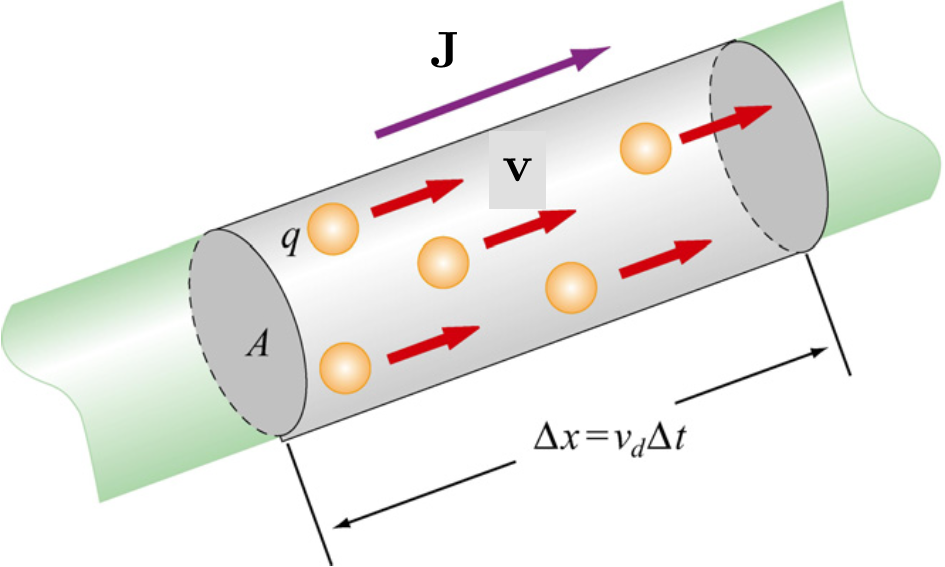
\includegraphics[scale=.3]{corrente_condutor}
\caption{\textit{Cargas elétrica fluindo no intervalo $\Delta\,x$ de um condutor com área de seção transversal $A$.}}
\label{fig.corre_condu}
\end{figure}
Observando a figura \ref{fig.corre_condu} que mostra uma corrente fluindo num condutor, onde $q$ é a carga elétrica de cada partícula, $n$ é quantidade de partículas num determinado volume do condutor e $\Delta\,x$ é o comprimento do mesmo, temos que a quantidade de carga nesse volume é $\Delta\,Q=n\,q\,(A\,\Delta\,x)$. Se as partículas se movem com velocidade $v$, então a posição a cada intervalo de tempo é dada por $\Delta\,x=v\,\Delta\,t$, e a corrente elétrica média nesse intervalo do condutor é
\begin{equation*}
I_m=\frac{\Delta\,Q}{\Delta\,t}=n\,q\,A\,v.
\end{equation*}
Como a densidade de corrente é a corrente média por área, temos que a mesma pode ser escrita como 
\begin{equation*}
\mathbf{J}=n\,q\,\mathbf{v}.
\end{equation*}

A terceira equação de Maxwell em sua forma integral pode ser obtida substituindo as equações \ref{eq.densidade_corrente} e \ref{eq.fluxo_eletrico} na equação \ref{eq.ampere_generalizada},
\begin{align*}
\oint_s\mathbf{B}\cdot d\mathbf{s}&=\mu_0I+\mu_0\epsilon_0\frac{d\phi_E}{dt}\\
\oint_s\frac{\mathbf{B}}{\mu_0}\cdot d\mathbf{s}&=\iint_S\mathbf{J}\cdot\,d\mathbf{A}+\frac{d}{dt}\oiint_S\epsilon_0\,\textbf{E}\cdot\textit{d}\textbf{A}
\end{align*}

A quarta e última equação de Maxwell é obtida substituindo a equação do fluxo magnético \ref{eq.fluxo_mag} na lei de Faraday \ref{eq.lei_faraday},
\begin{align*}
\oint_s\mathbf{E}\cdot d\mathbf{s}&=-\frac{d\phi_\mathbf{B}}{dt}\\
\oint_s\mathbf{E}\cdot d\mathbf{s}&=-\frac{d}{dt}\iint_S\mathbf{B}\cdot d\mathbf{A}.
\end{align*}

Todos os fenômenos eletromagnéticos são governados por essas quatro equações de Maxwell  e os últimos duzentos anos acumularam evidências suficientes para tal fato. Como vimos, todas as equações têm princípios experimentais, são deduzidas formalmente em termos de cálculo diferencial e integral, e são satisfeitas pelas variáveis físicas $\rho$ e $\mathbf{J}$ que são as fontes dos campos elétrico e magnético respectivamente. As equações são sumarizadas a seguir:
\begin{align}\label{eq.maxwell_1}
\oiint_S\epsilon_0\textbf{E}\cdot\textit{d}\textbf{A}&=\iiint_{V}\rho\,dV,\\\nonumber\\\label{eq.maxwell_2}
\oiint_S\textbf{B}\cdot\textit{d}\textbf{A}&=0,\\\nonumber\\\label{eq.maxwell_3}
\oint_s\frac{\mathbf{B}}{\mu_0}\cdot d\mathbf{s}&=\iint_S\mathbf{J}\cdot\,d\mathbf{A}+\frac{d}{dt}\oiint_S\epsilon_0\,\textbf{E}\cdot\textit{d}\textbf{A},\\\nonumber\\\label{eq.maxwell_4}
\oint_s\mathbf{E}\cdot d\mathbf{s}&=-\frac{d}{dt}\iint_S\mathbf{B}\cdot d\mathbf{A}.
\end{align}

\section{Generalizações da teoria}

\subsection{Ação do campo elétrico na matéria}

Nosso intuito é utilizar as equações de Maxwell para ajudar a determinar a composição de uma determinada região da subsuperfície. As informaçãoes sobre as propriedades eletromagnéticas de um material que compõe uma região dependem dos parâmetros $\rho$ e $\mathbf{J}$ de cada região, e esses parâmetros são usados para definir e inserir nas equações de Maxwell dois campos vetoriais, $\mathbf{D}$ e $\mathbf{H}$, que estão diretamente ligados às características do meio como veremos a seguir.

De acordo com \cite{griffiths}, um átomo eletricamente neutro também tem algumas de suas características alteradas quando expostos a campo elétrico $\mathbf{E}$, pois as cargas positivas (no núcleo) são empurradas numa direção e as cargas negativas (elétrons) são empurradas num sentido oposto. Na verdade, se o campo elétrico é muito forte, pode ser criada uma alteração permanente ``ionizando" o átomo. A aplicação de campo elétrico não tão extremo faz com que um equilíbrio seja rapidamente estabilizado criando um centro de cargas positivas e outro de cargas negativas deixando o átomo \textit{polarizado}, o qual agora passa a ter um pequeno \textit{momento de dipolo elétrico}, $\mathbf{p}$, que tem a mesma direção do campo elétrico e é proporcional ao mesmo.
\begin{equation*}
\mathbf{p}=\alpha\,\mathbf{E},
\end{equation*}
onde $\alpha$ é a constante de \textit{polarizabilidade atômica}. 

Numa substância dielétrica (isolante) qualquer quando exposta a um campo elétrico, cada átomo eletricamente neutro gera um pequeno momento de dipolo elétrico que se alinha como o campo aplicado. Se as moléculas já possuem naturalmente um momento de dipolo, todos eles experimentam um torque e também se alinham ao campo elétrico, assim a substância se torna polarizada e podemos definir a \textit{polarização} $\mathbf{P}$ de uma substância como o momento de dipolo elétrico por unidade de volume,
\begin{equation}
\mathbf{P}=\lim_{\Delta\,V\to 0}\frac{\mathbf{p}}{\Delta\,V}.
\end{equation}
\begin{figure}
\centering
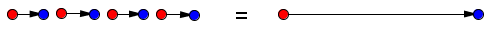
\includegraphics[scale=.7]{pequenos_dipolos}
\caption{\textit{As cargas em vermelho são negativas e em azul as positivas.}}
\label{fig.penquenos_dipolos}
\end{figure}
Suponha que temos uma longa cadeia de dipolos conforme a figura \ref{fig.penquenos_dipolos}, onde cada concentração de cargas se cancela com a concentração vizinha mas que ao final restarão duas concentrações de cargas opostas, como se vários pequenos deslocamentos resultassem num único deslocamento maior. As cargas nas extremidades são chamadas \textit{cargas de fronteira} e para calcular o acúmulo dessas cargas resultantes de uma polarização $\mathbf{P}$ vamos considerar um tubo feito de um material dielétrico paralelo a $\mathbf{P}$ de acordo com a figura \ref{fig.polari_cilindro}. 
\begin{figure}
\centering
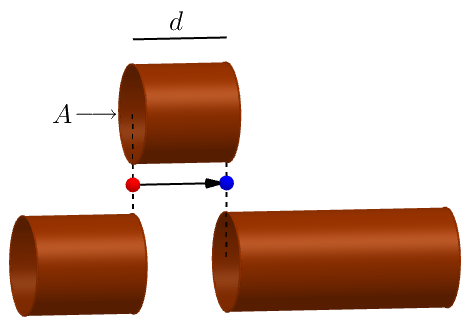
\includegraphics[scale=.5]{polarizacao_cilindro}
\caption{\textit{Momento de dipolo elétrico numa pequena amostra do cilindro.}}
\label{fig.polari_cilindro}
\end{figure}
Sendo $P$ a polarização de uma minúscula amostra do volume, $A$ a área de seção transversal do tubo e $d$ o comprimento da amostra, temos que o momento de dipolo da amostra é dado por $P\,A\,d$. Em termos de carga elétrica, esse momento de dipolo também pode ser definido como $q\,d$, onde $q$ é a carga elétrica no limite direito da amostra, e de onde se deduz que $q=P\,A$. Com a polarização, cargas são acumuladas no inteiror do corpo formando uma densidade de carga de polarização $\rho_p$, ocorrendo então um fenômeno de divergência da polarização através da superfície do tubo análago ao fenômeno da lei de Gauss. Assim, como um corpo dielétrico é eletricamente neutro, a quantidade total de carga negativa acumulada no interior do tubo é igual e oposta à quantidade de carga positiva empurrada através da superfície,
\begin{equation}\label{eq.polarizacao_densidade}
\iiint_V\rho_p\,d\,V=-\oiint_S\mathbf{P}\cdot d\mathbf{A}.
\end{equation}
Um meio não possui somente cargas de polarização mas também pode possuir \textit{cargas livres}, as quais se movimentam livremente sob a ação de um campo elétrico. Denotando por $Q_f$ a quantidade de cargas livres e $Q_p$ as cargas de polarização, temos que a quantidade total de cargas de um meio qualquer é dada por
\begin{equation*}
Q=Q_f+Q_p,
\end{equation*} 
e usando a equação \ref{eq.densidade_carga}, temos que a densidade de carga do meio é
\begin{equation}\label{eq.densi_carga_f_p}
\iiint_{V}\rho\,dV=\iiint_{V}\rho_f\,dV+\iiint_{V}\rho_p\,dV.
\end{equation}
Substituindo a equação \ref{eq.densi_carga_f_p} na equação \ref{eq.maxwell_1}, a lei de Gauss para o fluxo elétrico se torna
\begin{equation}\label{eq.lei_gauss_polarizacao}
\oiint_S\epsilon_0\,\mathbf{E}\cdot d\mathbf{A}=\iiint_{V}\rho_f\,dV+\iiint_{V}\rho_p\,dV.
\end{equation}
Substituindo a equação \ref{eq.lei_gauss_polarizacao} na equação \ref{eq.polarizacao_densidade}, temos uma relação entre as cargas livres e de polarização com a lei de Gauss,
\begin{align*}
\oiint_S\epsilon_0\,\mathbf{E}\cdot d\mathbf{A}&=\iiint_{V}\rho_f\,dV+\iiint_{V}\rho_p\,dV\\
\oiint_S\epsilon_0\,\mathbf{E}\cdot d\mathbf{A}&=\iiint_{V}\rho_f\,dV+\oiint_S\mathbf{P}\cdot d\mathbf{A}\\
\oiint_S\epsilon_0\,(\mathbf{E}-\mathbf{P})\cdot d\mathbf{A}&=\iiint_{V}\rho_f\,dV,
\end{align*}
onde a expressão $\mathbf{D}=\epsilon_0\,\mathbf{E}-\mathbf{P}$ é chamada \textit{campo de densidade de fluxo elétrico}, e por fim
\begin{equation*}
\oiint_S\mathbf{D}\cdot d\mathbf{A}=\iiint_{V}\rho_f\,dV.
\end{equation*}

Para muitas subst\^ancias, a polariza\c{c}\~ao \'e proporcional ao campo el\'etrico
\begin{equation*}
\mathbf{P}=\epsilon_0\chi_e\mathbf{E},
\end{equation*}
onde $\chi_e$ \'e a \textit{susceptibilidade el\'etrica} do meio e depende das caracter\'isticas deste, os quais s\~ao chamados \textit{diel\'etricos lineares}. Substituindo essa rela\c{c}\~ao na equa\c{c}\~ao do campo de desnidade de fluxo el\'etrico temos
\begin{align*}
\mathbf{D}&=\epsilon_0\mathbf{E}-\mathbf{P}\\
&=\epsilon_0\mathbf{E}-\epsilon_0\chi_e\mathbf{E}\\
&=\epsilon_0(1-\chi_e)\mathbf{E}\\
&=\epsilon\,\mathbf{E},
\end{align*}
e assim vemos que, para materiais diel\'etricos lineares, $\mathbf{D}$ tamb\'em \'e proporcional a $\mathbf{E}$, onde $\epsilon$ \'e chamado \textit{permissividade el\'etrica do meio}.

\subsection{A\c{c}\~ao de campo magn\'etico na mat\'eria}

Vimos na subseç\~ao \ref{sec.lei_ampere} que correntes el\'etricas geram campos magn\'eticos, mas na verdade todos os fen\^omenos magn\'eticos são devidos a cargas el\'etricas em movimento. Se examinarmos um material magn\'etico qualquer em n\'ivel at\^omico, encontraremos pequenas correntes, as do el\'etron orbitando o n\'ucleo do \'atomo e a rota\c{c}\~ao de cada el\'etron em torno de seu pr\'oprio eixo. Em termos macrosc\'opicos essas correntes em la\c{c}os s\~ao t\~ao pequenos que s\~ao tratados como o \textit{momento de dipolo magn\'etico}, $\mathbf{m}$, similar ao que foi feito para o momento de dipolo el\'etrico. Quando um campo magn\'etico externo \'e aplicado ocorre o alinhamento desses dipolos magn\'eticos e o corpo se torna magneticamente polarizado ou \textit{magnetizado}. O estado de polariza\c{c}\~ao magn\'etica de um material \'e medido pelo momento de dipolo magn\'etico por unidade infinitesimal de volume, ou \textit{magnetiza\c{c}\~ao}
\begin{equation*}
\mathbf{M}=\lim_{\Delta\,V\to 0}\frac{\mathbf{m}}{\Delta\,V}.
\end{equation*}   
A densidade de corrente el\'etrica pode ser composta pelas \textit{densidade de correntes livres} $\mathbf{J}_f$, \textit{densidade de correntes de polariza\c{c}\~ao} $\mathbf{J}_p$ e \textit{densidade de correntes de magnetiza\c{c}\~ao} $\mathbf{J}_m$. Quando a magnetiza\c{c}\~ao de um material \'e uniforme, as correntes dos la\c{c}os internos (sem considerar a superf\'icie) se cancelam e n\~ao h\'a a gera\c{c}\~ao de densidade de correntes de magnetiza\c{c}\~ao, e quando a magnetiza\c{c}\~ao \'e n\~ao uniforme a diferen\c{c}a entre as correntes em cada la\c{c}o faz com que $\mathbf{J}_m$ seja diferente de zero. Na figura \ref{fig.magnetizacao} eh apresentado um exemplo com duas amostras infinitesimais de um material juntamente com os vetores que indicam a intensidade e a dire\c{c}\~ao da magnetiza\c{c}\~ao, e os tri\^angulos que indicam o sentido e intensidade da corrente.
\begin{figure}
\centering
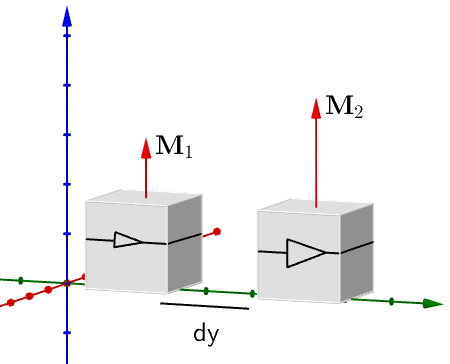
\includegraphics[scale=.5]{magnetizacao}
\caption{\textit{A magnetiza\c{c}\~ao n\~ao uniforme produz densidade de corrente de magnetiza\c{c}\~ao.}}
\label{fig.magnetizacao}
\end{figure}     
Nas superf\'icies onde as amostras se juntam a corrente final na dire\c{c}\~ao do eixo $x$ \'e dada pela diferen\c{c}a entre as correntes em cada amostra, geradas por suas respectivas magnetiza\c{c}\~oes na dire\c{c}\~ao do eixo $z$. Analogamente, sendo a magnetizacao no sentido do eixo $y$, a corrente resultante tamb\'em ser\'a na dire\c{c}\~ao do eixo $x$ mas em sentido oposto. Usando essa diferen\c{c}a de sentido das correstes resultantes e a equa\c{c}\~ao \ref{eq.densidade_corrente} podemos demonstrar que a densidade de corrente de magnetiza\c{c}\~ao \'e dada por
\begin{equation}\label{eq.magnetizacao_densi_corrente}
\iint_S\mathbf{J}_m\cdot d\,\mathbf{A}=\oint_s \mathbf{M}\cdot d\,\mathbf{s}.
\end{equation}


Se a concentra\c{c}\~ao de cargas em um volume muda, ent\~ao essa diferen\c{c}ca entre a quantidade inicial e a final tem que ter passado pela superf\'cie (saindo ou entrando) que engloba o volume. Assim, a varia\c{c}\~ao no tempo de uma quantidade carga saindo de um certo volume \'e igual a corrente que atravessa a superf\'icie desse volume. Considerando a densidade de cargas e correntes de polariza\c{c}\~ao, e usando as equa\c{c}\~oes \ref{eq.densidade_carga} e \ref{eq.densidade_corrente}, temos
\begin{align*}
\frac{d\,Q}{d\,t}&=-\iint_S\mathbf{J}_p\cdot d\mathbf{A}\\
\iiint_V\frac{\partial}{\partial\,t}\rho_p\,dV&=-\iint_S\mathbf{J}_p\cdot d\mathbf{A}.
\end{align*}
Mas, pela equa\c{c}\~ao \ref{eq.polarizacao_densidade}, podemos escrever
\begin{equation}\label{eq.polarizacao_densi_corrente}
\iint_S\mathbf{J}_p\cdot d\mathbf{A}=\oiint_S\mathbf{P}\cdot d\mathbf{A}.
\end{equation} 
Considerando os tr\^es tipos de densidade de correntes, $\mathbf{J}_f$, $\mathbf{J}_p$ e $\mathbf{J}_m$, podemos escrever a lei de Amp\`ere generalizada dada pela equa\c{c}\~ao \ref{eq.maxwell_3} na forma
\begin{align*}
\oint_s\frac{\mathbf{B}}{\mu_0}\cdot d\mathbf{s}&=\\iint_S\mathbf{J}\cdot\,d\mathbf{A}+\frac{d}{dt}\oiint_S\epsilon_0\,\textbf{E}\cdot\textit{d}\textbf{A}\\\\
\oint_s\frac{\mathbf{B}}{\mu_0}\cdot d\mathbf{s}-\frac{d}{dt}\oiint_S\epsilon_0\,\textbf{E}\cdot\textit{d}\textbf{A}&=\iint_S\mathbf{J}_f\cdot\,d\mathbf{A}+\iint_S\mathbf{J}_p\cdot\,d\mathbf{A}+\iint_S\mathbf{J}_m\cdot\,d\mathbf{A}.
\end{align*}
Substituindo as equa\c{c}\~oes \ref{eq.magnetizacao_densi_corrente} e \ref{eq.polarizacao_densi_corrente}, podemos reescrever a lei de Amp\`ere generalizada como
\begin{align*}
\oint_s\frac{\mathbf{B}}{\mu_0}\cdot d\mathbf{s}-\frac{d}{dt}\oiint_S\epsilon_0\,\textbf{E}\cdot\textit{d}\textbf{A}&=\iint_S\mathbf{J}_f\cdot\,d\mathbf{A}+\oiint_S\mathbf{P}\cdot d\mathbf{A}+\oint_s \mathbf{M}\cdot d\,\mathbf{s}\\\\
\oint_s(\frac{\mathbf{B}}{\mu_0}-\mathbf{M})\cdot d\mathbf{s}&=\iint_S\mathbf{J}_f\cdot\,d\mathbf{A}+\frac{d}{dt}\oiint_S(\epsilon_0\,\textbf{E}+\mathbf{P})\cdot\textit{d}\textbf{A},
\end{align*}
onde $\frac{1}{\mu_0}\mathbf{B}-\mathbf{M}=\mathbf{H}$ \'e definido como o \textit{campo magn\'etico auxiliar}. Em atividades experimentais \'e mais f\'acil medir o campo 
$\mathbf{E}$ a partir da aplica\c{c}\~ao de uma diferen\c{c}a de potencial num circuito el\'etrico do que medir o campo $\mathbf{D}$ a partir da concentra\c{c}\~ao de cargas el\'etricas. Com o campo $\mathbf{H}$ acontece o contr\'ario, \'e mais f\'acil medi-lo a partir da corrente el\'etrica numa bobina do que medir o campo magn\'etico $\mathbf{B}$, j\'a que este \'ultimo depende do tipo de material usado. Portanto, alguns pesquisadores e autores costumam chamar $\mathbf{H}$ de campo magn\'etico e $\mathbf{B}$ de campo de densidade de fluxo magn\'etico, mas esta \'ultima defini\c{c}\~ao, como vimos, pode se confundir com outro tipo de medida, $\phi_\mathbf{B}$.

Para algumas subst\^ancias, a magnetiza\c{c}\~ao \'e proporcional ao campo magn\'etico auxiliar
\begin{equation*}
\mathbf{M}=\chi_m\mathbf{H},
\end{equation*}
onde $\chi_m$ \'e a \textit{susceptilidade magn\'etica do meio} e depende das caracter\'isticas deste. Substituindo essa \'ultima equa\c{c}\~ao na equa\c{c}\~ao do campo magn\'etico auxiliar temos
\begin{align*}
\mathbf{B}&=\mu_0\,(\mathbf{H}+\mathbf{M})\\
&=\mu_0\,(\mathbf{H}+\chi_m\mathbf{H})\\
&=\mu_0\,(1+\chi_m)\,\mathbf{H}\\
&=\mu\,\mathbf{H},
\end{align*}
onde $\mu$ \'e a \textit{permeabilidade magn\'etica do meio}.

Assim, podemos escrever as equa\c{c}\~oes de Maxwell considerando a a\c{c}\~ao dos campos el\'etrico e magn\'etico na mat\'eria como
\begin{align}\label{eq.max_meio_1}
\oiint_S\mathbf{D}\cdot d\mathbf{A}&=\iiint_{V}\rho_f\,dV,\\\nonumber\\\label{eq.max_meio_2}
\oiint_S\textbf{B}\cdot\textit{d}\textbf{A}&=0,\\\nonumber\\\label{eq.max_meio_3}
\oint_s\mathbf{H}\cdot d\mathbf{s}&=\iint_S\mathbf{J}_f\cdot\,d\mathbf{A}+\frac{d}{dt}\oiint_S\mathbf{D}\cdot\textit{d}\textbf{A},\\\nonumber\\\label{eq.max_meio_4}
\oint_s\mathbf{E}\cdot d\mathbf{s}&=-\frac{d}{dt}\iint_S\mathbf{B}\cdot d\mathbf{A}.
\end{align}

\subsection{Forma diferencial das Equa\c{c}oes de Maxwell}

Experimentalmente tem-se obtido excelentes resultados aplicando as equa\c{c}\~oes de Maxwell em sua forma diferencial, onde s\~ao assumidas algumas hip\'oteses acerca da diferenciabilidade dos campos envolvidos. Utilizando essas hip\'oteses, podemos transcrever as equa\c{c}\~oes da forma integral para a forma diferencial.

Portanto, considerando uma regi\~ao fechada do espa\c{c}o $\mathbb{R}^3$ de volume $V$ e limitada pela superf\'icie $A$, temos pela equa\c{c}\~ao \ref{eq.max_meio_1} que
\begin{equation*}
\oiint_S\mathbf{D}\cdot d\mathbf{A}=\iiint_{V}\rho_f\,dV.
\end{equation*}
Supondo que o campo de densidade de fluxo el\'etrico seja de classe $C^1$, podemos usar o teorema da Diverg\^encia
\begin{equation*}
\oiint_S\mathbf{D}\cdot d\mathbf{A}=\iiint_V\nabla\cdot\mathbf{D}\,dV,
\end{equation*}
e realizar a substitui\c{c}\~ao
\begin{equation*}
\iiint_V\nabla\cdot\mathbf{D}\,dV=\iiint_{V}\rho_f\,dV.
\end{equation*}
Como a rela\c{c}\~ao acima \'e v\'alida para qualquer volume $V$ e supondo $\rho_f$ cont\'inuo, podemos reescrever a primeira equa\c{c}\~ao de Maxwell como
\begin{equation*}
\nabla\cdot\mathbf{D}=\rho_f.
\end{equation*}

Analogamente \`a situa\c{c}\~ao anterior, usando ainda o teorema da Diverg\^encia e supondo que o campo magn\'etico $\mathbf{B}$ seja de classe $C^1$, podemos escrever a segunda equa\c{c}\~ao de Maxwell, equa\c{c}\~ao \ref{eq.max_meio_2}, como
\begin{align*}
\iiint_V\nabla\cdot\mathbf{B}\,dV&=0\\\\
\nabla\cdot\mathbf{B}&=0.
\end{align*}

Utilizando o teorema de Stokes e considerando que o campo  magn\'etico auxiliar $\mathbf{H}$ seja de classe $C^1$, temos
\begin{equation*}
\oint_s\mathbf{H}\cdot d\mathbf{s}=\iint_S(\nabla\times\mathbf{H})\,d\mathbf{A}.
\end{equation*}
Supondo que a superf\'icie $A$ seja constante no tempo, podemos substituir a express\~ao anterior na lei de Amp\`ere-Maxwell (equa\c{c}\~ao \ref{eq.max_meio_3}) para chegar a
\begin{equation*}
\iint_S(\nabla\times\mathbf{H})\,d\mathbf{A}-\oiint_S\frac{\partial}{\partial t}\,\mathbf{D}\cdot d\mathbf{A}=\iint_S\mathbf{J}_f\,\cdot d\mathbf{A}.
\end{equation*}
Matematicamente n\~ao podemos usar a arbitrariedade de escolha da superf\'icie $A$, mas resultados experimentais tem sustentado que, de fato,
\begin{equation*}
\nabla\times\mathbf{H}-\frac{\partial}{\partial t}\,\mathbf{D}=\mathbf{J}_f.
\end{equation*}

Com desenvolvimento similar ao anteiror, podemos deduzir que a forma diferencial da quarta equa\c{c}\~ao de Maxwell, equa\c{c}\~ao \ref{eq.max_meio_4}, \'e
\begin{equation*}
\nabla\times\mathbf{E}=-\frac{\partial}{\partial t}\mathbf{D}.
\end{equation*}

Sumarizando as equa\c{c}\~oes de Maxwell em suas formas diferenciais e considerando as propriedades eletromagn\'eticas do meio, temos
\begin{align}
\nabla\cdot\mathbf{D}&=\rho_f,\\\nonumber\\
\nabla\cdot\mathbf{B}&=0,\\\nonumber\\
\nabla\times\mathbf{H}&=\mathbf{J}_f+\frac{\partial}{\partial t}\,\mathbf{D},\\\nonumber\\
\nabla\times\mathbf{E}&=-\frac{\partial}{\partial t}\mathbf{D}.
\end{align} 

\subsection{Condi\c{c}\~oes de Contorno entre Meios de Diferentes Composi\c{c}\~oes}

Segundo \cite{jackson_classical_1999}, as equa\c{c}\~oes de Maxwell em suas formas integrais (\ref{eq.max_meio_1} \`a \ref{eq.max_meio_4}) podem ser usadas para dedu\c{c}\~ao de rela\c{c}\~oes envolvendo as componentes tangenciais e normais dos campos el\'etrico e magn\'etico em ambos os lados da superf\'icie de contato entre dois meios com caracter\'isticas eletromagn\'eticas diferentes. Para a utiliza\c{c}\~ao das equa\c{c}\~oes \ref{eq.max_meio_1} e \ref{eq.max_meio_2}, consideramos um cilindro com altura infinitesimal onde cada uma de suas bases circulares pertencem a uma das camadas em quest\~ao. E para estudar as equa\c{c}\~oes \ref{eq.max_meio_3} e \ref{eq.max_meio_4}, utilizamos um circuito retangular tamb\'em de altura infinitesimal com cada um dos lados maiores pertencentes a uma das camadas. O esquema geom\'etrico dessa abordagem pode ser visto na figura tal. 

Como a altura do cilindro tende a zero, a superf\'icie lateral do cilindro n\~ao contribui para o c\'alculo da integral do lado esquerdo da equa\c{c}\~ao \ref{eq.max_meio_1}, onde tal contribui\c{c}\~ao \'e devida somente \`as \'areas das bases que s\~ao paralelas entre si e tangentes a superf\'icie que separa as duas camadas. Nessas condi\c{c}\~oes temos
\begin{equation*}
\oiint_S\mathbf{D}\cdot d\mathbf{A} = (\mathbf{D}_2-\mathbf{D}_1)\cdot\mathbf{n}\,\Delta A,
\end{equation*}
onde $\mathbf{D}_i$ \'e o campo de densidade de fluxo el\'etrico nas camadas 1 e 2, e $\mathbf{n}$ \'e o vetor normal \`a superf\'icie infinitesimal $dA$. Se a densidade volum\'etrica de carga \'e singular na superf\'icie de contato de forma a produzir uma densiddade de carga superficial, $\sigma$, ent\~ao a integral do lado direito da equa\c{c}\~ao \ref{eq.max_meio_1} fica
\begin{equation*}
\iiint_V\rho_f\,dV=\sigma\,\Delta A.
\end{equation*}
Assim, a componente normal da diferen\c{c}a entre os campos de densidade de fluxo el\'etrico em cada camada \'e dado por
\begin{equation*}
(\mathbf{D}_2-\mathbf{D}_1)\cdot\mathbf{n}=\sigma. 
\end{equation*} 
Usando a defini\c{c}\~ao de \textit{salto} da componente normal de um campo dada por \cite{erigen_1963} temos
\begin{equation}\label{eq.gau_meio_1}
(\mathbf{D}_2-\mathbf{D}_1)\cdot\mathbf{n}=\left[\left[\mathbf{D}\right]\right]\cdot\mathbf{n}=\sigma.
\end{equation}

Analogamente, podemos determinar o salto da componente normal do campo magn\'etico a partir da equa\c{c}\~ao \ref{eq.max_meio_2},
\begin{equation*}
(\mathbf{B}_2-\mathbf{B}_1)\cdot\mathbf{n}=\left[\left[\mathbf{B}\right]\right]\cdot\mathbf{n}=0.
\end{equation*}  
Ou seja, a componente normal do campo magn\'etico \'e cont\'inua na transi\c{c}\~ao das camadas, e a descontinuidade da componente normal do campo de densidade de fluxo el\'etrico \'e igual a densidade superficial de carga no ponto de transi\c{c}\~ao.

Agora vamos utilizar um circuito Stokesiano para determinar as componentes tangenciais \`a superf\'icie dos campos el\'etrico e magn\'etico auxiliar. Considerando desprez\'ivel a altura em rela\c{c}\~ao \`a superf\'icie do circuito retangular, e que seus outros dois lados s\~ao paralelos e t\^em comprimento $\Delta l$, ent\~ao o lado esquerdo da equa\c{c}\~ao \ref{eq.max_meio_3} \'e calculado como
\begin{equation}\label{eq.amp_meio_1}
\oint_s\mathbf{H}\cdot d\mathbf{s}=(\mathbf{H}_2-\mathbf{H}_1)\cdot(\mathbf{n}\times\mathbf{t})\Delta l.
\end{equation}
As integrais do lado direito da equa\c{c}\~ao \ref{eq.max_meio_3} n\~ao zeram se h\'a uma densidade de corrente superficial circulando na superf\'icie de contato. Nessas circunst\^ancias podemos escrever
\begin{equation}\label{eq.amp_meio_2}
\iint_S\mathbf{J}_f\cdot\,d\mathbf{A}+\frac{d}{dt}\oiint_S\mathbf{D}\cdot\textit{d}\textbf{A}=\mathbf{K}\cdot\mathbf{t}\,\Delta l+0,
\end{equation}
onde $\mathbf{K}$ \'e a densidade de corrente superficial, e $\mathbf{t}$ \'e o vetor tangente \`a superf\'icie de contato entre as camadas, e normal \`a \'area do circuito retangular. A segunda parcela \'e zero pois a varia\c{c}\~ao no tempo do campo de densidade de fluxo el\'etrico atrav\'es de uma superf\'icie \'e finita, e a superf\'icie em quest\~ao (circuito retangular) \'e zero quando sua altura tende a zero. Igualando os resultados das equa\c{c}\~oes \ref{eq.amp_meio_1} e \ref{eq.amp_meio_2} e aplicando as regras da an\'alise vetorial temos
\begin{equation}\label{eq.far_meio_1}
\mathbf{n}\times(\mathbf{H}_2-\mathbf{H}_1)=\left[\left[\mathbf{H}\right]\right]=\mathbf{K}.
\end{equation}
Similarmente ao desenvolvimento para o salto do campo magn\'etico auxiliar, temos o salto do campo el\'etrico deduzido a partir da equa\c{c}\~ao \ref{eq.max_meio_4},
\begin{equation}\label{eq.far_meio_2}
\mathbf{n}\times(\mathbf{E}_2-\mathbf{E}_1)=\left[\left[\mathbf{E}\right]\right]=0.
\end{equation}
O lado esquerdo da equa\c{c}\~ao acima \'e zero pelo mesmo argumento dado anteriormente. A varia\c{c}\~ao no tempo de um campo magn\'etico finito atrav\'es de uma superf\'icie retangular nula, pois sua altura tende a zero.
Pela equa\c{c}\~ao \ref{eq.far_meio_1} temos que a densidade de corrente superficial tem somente componentes paralelas \`a superf\'icie de contato entre as camadas, e a componente tangencial do campo magn\'etico auxiliar \'e descontinua por uma quantidade cuja magnitude \'e igual \`a magnitude da densidade de corrente superficial e cuja dire\c{c}\~ao \'e paralela ao vetor $\mathbf{K}\times\mathbf{n}$. Pela equa\c{c}\~ao \ref{eq.far_meio_2} temos que a componente tangencial do capo el\'etrico atrav\'es da interface \'e continua. As deconstinuidades apresentadas nas equa\c{c}\~oes \ref{eq.gau_meio_1} e \ref{eq.far_meio_1} s\~ao prestativas para resolver as equa\c{c}\~oes de Maxwell em diferentes regi\~oes e conectar as solu\c{c}\~oes para obter campos para qualquer lugar do espa\c{c}o.  






\section{Conclusões}